% !TEX root = ../TAMU_Thesis_Main.tex

%%%%%%%%%%%%%%%%%%%%%%%%%%%%%%%%%%%%%%%%%%%%%%%%%%%%%%%%%%%%%%%%%%%%%%%
%%%                           SECTION II
%%%%%%%%%%%%%%%%%%%%%%%%%%%%%%%%%%%%%%%%%%%%%%%%%%%%%%%%%%%%%%%%%%%%%%


\chapter[footnote={This paper is published in \textit{Journal of Advances in Modeling Earth System}. Reprinted with permission from American Geophysical Union. Full citation:  Schlichting, D., Qu, L., Kobashi, D., \& Hetland, R. (2023). Quantification of physical and numerical mixing in a coastal ocean model using salinity variance budgets. Journal of Advances in Modeling Earth Systems, 15, e2022MS003380. \url{ https://doi.org/10.1029/2022MS003380}}]{Quantification of Physical and Numerical Mixing in a Coastal Ocean Model Using Salinity Variance Budgets}

\section{Abstract}
Numerical mixing, the spurious mixing primarily generated by the discretization of advection, is often significant in estuarine and coastal models due to sharp, energetic fronts. We compare on- and offline estimates of numerical mixing in a submesoscale-resolving realistic simulation of the ocean state over the Texas-Louisiana continental shelf. While offline estimates of numerical mixing differ from online estimates, offline methods may be the only analysis available. We use two methods to estimate numerical mixing offline based on the residuals of the salinity squared $s^2$ and volume-mean salinity variance $s^{\prime^2}$ budgets. The $s^{\prime^2}$ budget overestimates the time-averaged online numerical mixing by 60\% at hourly output. The $s^2$ budget compares poorly due to large truncation errors associated with the tendency and advection terms. The residual of the $s^2$ budget starts to converge to the $s^{\prime^2}$ budget as output frequency increases to 10 minutes -- an unrealistic frequency for long-term coastal ocean simulations -- but neither method unconditionally converges to the online method and therefore cannot be recommended for generic analysis of numerical mixing. We also investigate the effects of horizontal resolution on numerical mixing using a two-way nested grid with the online method. The volume-integrated numerical mixing constitutes 57\% of the bulk physical mixing -- the mixing prescribed by the turbulence closure scheme -- in the coarse model and may exceed the physical mixing by half an order of magnitude. We find numerical mixing is reduced by 35\% on average in the nested model, likely due to new dynamical processes that emerge in the nested simulation.

\section{Plane language summary}
Numerical models are powerful tools for studying the general circulation of the ocean, allowing us to examine the ocean's complex relationship with Earth's weather and climate in greater detail than observations allow. However, numerical ocean models are prone to several types of numerical errors because they represent physical processes with discrete approximations. One of these errors is numerical mixing, a process by which the discretized transport of tracers by currents generates spurious mixing. Recent studies suggest numerical mixing can be as large as the physical mixing prescribed by a parameterization, especially in regions with strong tracer gradients, such as in estuaries or the coastal ocean. In this study, we examine numerical salinity mixing using a combination of on- and offline methods in a model of the ocean state over the Texas-Louisiana continental shelf in the Gulf of Mexico. Offline methods rely on existing model output and are often easier to implement than online methods. However, offline methods trade numerical accuracy for convenience because online methods require modifying a model's source code and re-running it. We find offline estimates of numerical mixing should not be used because they may be inaccurate even at impractically high resolution.

\section{Introduction}
Mixing is an irreversible process that redistributes tracers and dissipates energy. In primitive equation ocean models, turbulence closure schemes are used to parameterize the physical mixing due to subgrid-scale turbulence. In addition to the prescribed physical mixing, spurious or numerical mixing may be generated by several sources, such as the discretization of the advective terms in the momentum and tracer equations \citep{Burchard_2008, gibson2017attribution, Griffies_2000, Smolarkiewicz_1983}, spurious convection due to grid-scale noise \citep{ilicak2016quantifying,Ilicak_2012}, and cabbeling that arises from the nonlinear equation of state for seawater density \citep{Ilicak_2012, mcdougall1987thermobaricity}. Numerical mixing induces spurious diffusion or anti-diffusion of tracer gradients, which affects the tracer distribution and may introduce biases in the tracer field \citep{Holmes_2021}. Numerical mixing is often significant in regions with strong velocity shear and tracer gradients \citep{Fringer_2019, Kalra_2019, Rennau_2009}, however, it is seldom quantified in realistic simulations of estuarine and coastal flows \citep{Broatch_2022, Ralston_2017, Wang_2021}.

This study is focused on quantifying the magnitude of spurious mixing -- in particular, the numerical mixing generated by the discretization of tracer advection -- distinct from the prescribed mixing specified through mixing closure parameterizations regardless of the accuracy of these closure models; that is to say, spurious mixing that cannot be directly controlled by model configuration. For example, errors in physical mixing relative to a true ocean state may arise when using a grid or geopotential aligned horizontal diffusion tensor, instead of rotating the diffusion tensor to align with the isoneutral directions \citep{griffies1998isoneutral, redi1982oceanic}. However, a mixing tensor aligned with geopotentials is still something that is specified --  an explicit parameterization of unresolved processes, albeit poorly or incorrectly -- and can be controlled in the model setup; such parameterizations are considered to be ``prescribed", even if unphysical, for purposes of this study.

In limited-domain coastal ocean simulations, explicit horizontal mixing is commonly kept as low as possible, ideally with no explicit horizontal mixing, allowing a flux-limiting \citep{Smolarkiewicz_1998} or upwind \citep{shchepetkin1998quasi} tracer advection scheme to prevent the accumulation of variance at the grid scale. This has the advantage that mixing, in the form of numerical diffusion, is strongest in the regions where tracer gradients are large but is small elsewhere. Tracer distributions across energetic fronts remain monotonic, and weaker tracer gradients associated with less energetic features remain persistent, resulting in tracer fields that, for example, have the same qualitative structures as remotely sensed sea surface temperature or other optical water properties. As such, advection schemes that can cause significant, but targeted, numerical diffusion are important tools in modern coastal oceanography. However, a disadvantage of this approach is that it is difficult to control and quantify the amount of mixing within the simulation.

Numerical methods have been developed for quantifying numerical mixing online during the model run based on tracer variance dissipation \citep{Burchard_2008, Klingbeil_2014}, water mass transformation \citep{Holmes_2021, lee2002spurious, megann2018estimating}, and energetics \citep{Ilicak_2012, Petersen_2015, winters1995available}. However, online methods are not always practical because they require modifying a model's source code and rerunning it, or may be unavailable when downloading model output from an external source. Consequently, offline methods for quantifying numerical mixing based on tracer variance budgets have become increasingly popular among estuarine and coastal modelers \citep{Li_2018, MacCready_2018, Wang_2017, Wang_2021}, who often use salinity as the tracer of interest because it dominates the density structure in many coastal regions. Salinity distributions are also strongly controlled by lateral advection -- and thus more susceptible to errors in the advection scheme -- since salinity structure in coastal regions is primarily driven by lateral boundary conditions (e.g., rivers) rather than surface boundary conditions (e.g., precipitation and evaporation). 

We use a subset of a submesoscale-resolving ocean model of the Texas-Louisiana (TXLA) continental shelf in the northern Gulf of Mexico (nGoM) during summer as a case study, where the density field is dominated by salinity variations due to freshwater input from the Mississippi and Atchafalaya rivers. This region is known to have an energetic eddy field \citep{Hetland_2017} and intense fronts \citep{qu2022rapid}. Understanding the circulation and mixing in this region is important for better predictions of along-coast connectivity and constituent transport \citep{thyng2023seasonal}, seasonal hypoxia \citep{Xomchuk_2020, zhang2015processes}, and the shelf ecosystem \citep{fennel2011coupled}. We also want to understand the sensitivity of numerical mixing to resolution, so we use a two-way nested child model with five times the parent resolution to test the sensitivity of numerical mixing to horizontal grid resolution. 

\subsection{Quantifying physical mixing}

Physical mixing can be defined as the dissipation of salinity variance, $\chi^s$, due to molecular processes \citep{Burchard_2009}, which is analogous to the dissipation of turbulent kinetic energy $\epsilon$ \citep{MacCready_2018}. $\epsilon$ represents the rate at which kinetic energy is dissipated by molecular viscosity and has units of velocity squared per unit time (m$^2$ s$^{-3}$). $\chi^s$ represents the rate at which salinity variance is dissipated by molecular diffusion \citep{Nash_2002} and has units of salinity squared per unit time (g$^2$ kg$^{-2}$ s$^{-1}$). The molecular dissipation of salinity variance is assumed to be equal to, on average, the dissipation of Reynolds averaged salinity variance at the scales of the turbulent eddies \citep{Burchard_2008, Nash_2002, osborn1972oceanic}, and may be written as

\begin{equation} \label{eq:chi_whole}
    \chi^s = 2 \overline{s^\prime \mathbf{u}^\prime} \cdot \nabla s = \underbrace{2\kappa_H \left[\left(\frac{\partial s}{\partial x}\right)^2 + \left(\frac{\partial s}{\partial y} \right)^2 \right]}_{\text{Horz. mixing $\chi_H^s$}}+\underbrace{2 \kappa_s \left(\frac{\partial s}{\partial z} \right)^2}_{\text{Vert. mixing $\chi_v^s$}}
\end{equation}
where $s$ is the salinity, $\mathbf{u}$ is the 3D velocity vector, an overbar is used to denote a Reynolds average, and a prime is used to denote a perturbation from that average. The physical mixing resolved by a model is quantified as the dissipation of Reynolds averaged salinity variance with the eddy diffusivity $\kappa$. Due to the vast differences in the horizontal and vertical scales in the ocean, $\kappa$ is separated into horizontal ($\kappa_H$) and vertical ($\kappa_s$) components and thus requires different parameterizations. $\kappa_H$ is parameterized by the horizontal mixing scheme and $\kappa_s$ parameterized by the turbulence closure scheme \citep{Burchard_2008, MacCready_2018}. 

As discussed above, in many estuarine and coastal models, if $\kappa_H$ is prescribed, it is often done with the smallest possible values to reduce spurious noise in the salinity field. Consequently, the horizontal mixing $\chi_H^s$ is often much smaller \citep{geyer2014estuarine} than the vertical mixing $\chi_v^s$, with some exceptions \citep{Broatch_2022}. While this is different than many larger-scale ocean circulation models, we consider horizontal mixing as part of the physical mixing because it is prescribed, whereas numerical mixing is not something that can be directly controlled in the model setup. Generally, horizontal and vertical down-gradient closure models -- including parameterizations of vertical shear mixing, harmonic, and biharmonic lateral mixing -- result in a positive definite $\chi^s$ that represents a sink of salinity variance.

\subsection{Quantifying numerical mixing}

Salinity variance budgets provide a means to quantify the bulk physical and numerical mixing within a control volume \citep{Li_2018, Lorenz_2021, Qu_2022_box}. Numerical models are designed to conserve salinity, but not salinity variance, therefore numerical mixing is treated as an additional subgrid-scale term and quantified as the residual of the salinity variance budget \citep{MacCready_2018}. Salinity variance can be defined with or without reference to a volume mean \citep{Burchard_2008, Qu_2022_box}, with the former denoted hereinafter as the volume-mean salinity variance $s^{\prime^2} = (s-\overline{s})^2$, where $\overline{s}$ is the volume-averaged salinity $\frac{1}{V} \iiint s \, dV$, and the latter denoted as the salinity squared $s^2$. For example, consider a three-dimensional control volume with no external sources or sinks of volume-mean salinity variance (i.e., no surface salt fluxes or horizontal diffusive boundary fluxes). The numerical mixing $\mathcal{M}_{num}$ based on the volume-integrated $s^{\prime^2}$ budget is

\begin{equation} \label{eq:svar_maccready}
    \mathcal{M}_{num} = \mathcal{D} \biggl\{-\frac{d}{dt} \iiint_V s^{\prime^2} dV - \iint_{A_l} \mathbf{u}s^{\prime^2} \cdot \hat{\mathbf{n}} \,  dA - \iiint_V \chi^s \, dV \biggl\} \quad ,
\end{equation}
where $\mathcal{D}$ denotes a generic discretization operator, $t$ denotes time, $V$ denotes the domain volume, $A_l$ denotes the area of the lateral control volume boundaries, $\mathbf{u}$ is the velocity normal to the open boundaries, $\hat{\mathbf{n}}$ is the outward pointing normal vector, and $\chi^s$ is the physical mixing as defined in the right-hand-side (RHS) of Eq. \ref{eq:chi_whole}. Eq. \ref{eq:svar_maccready} is modified version of Eq. 3 of \citet{MacCready_2018}. We have written the volume-mean salinity variance budget inside of a discretization operator because numerical mixing only appears as a consequence of discretization. As with the physical mixing, the numerical mixing is assumed to be a sink of salinity variance (the reasons for this will become more apparent in Section \ref{sec:theory}), which is reflected in the sign convention of the RHS terms. Eq. \ref{eq:svar_maccready} demonstrates that in the absence of diffusive fluxes, contributions to numerical mixing arise from the time rate of change of variance within the control volume, the advection of variance through the lateral boundaries, and the dissipation of variance due to turbulent mixing. 

A salinity variance budget based on $s^{\prime^2}$ \citep{Li_2018} showed that the volume-mean salinity variance may be used as a tracer for the stratification within a control volume, an approach that inspired later studies \citep{Broatch_2022, Li_2021, Wang_2018}. Conversely, \citet{Lorenz_2021} and \citet{Burchard_2019} derived a series of approximate relations for the total mixing within a control volume based on the $s^2$ budget because it is easier to apply to model output and field observations than the $s^{\prime^2}$ budget. There are a number of examples where mixing within a control volume is estimated by the boundary fluxes. The bulk mixing $M$ in an estuary may be approximated as $M=s_{in}s_{out}Q_r$ \citep{Burchard_2019, Burchard_2020}, where $s_{in}$ and $s_{out}$ are the inflowing and outflowing salinities calculated with the total exchange flow (TEF) analysis framework \citep{MacCready_2011}, respectively, and $Q_r$ is the river discharge. Under the same assumptions, \citet{Qu_2022_box} showed that $M$ be quantified directly in terms of the net boundary advection of salinity variance into the estuary. Due to the recent invention of the theory, TEF has only been applied to numerical model output. However, a recent paper by \citet{Lemagie_2022} suggested how TEF may be measured with field observations. 

Without a robust estimate of $\overline{s}$ for many estuaries and coastal regions, it may be feasible to only estimate the advective boundary fluxes of $s^2$. Consequently, there is strong motivation to explore how $s^2$ and $s^{\prime^2}$ are related. Despite the physical mixing being identical in the $s^2$ and $s^{\prime^2}$ budgets (since $\overline{s}$ has no spatial gradients), this is not necessarily true for other terms (e.g., advection) in their respective equations. This is particularly relevant for realistic, unsteady flows within control volumes characterized by advective and diffusive lateral boundary fluxes, and surface salt fluxes caused by evaporation and precipitation. Therefore, it is unclear \textit{a priori} if the $s^2$ budget may be used to robustly estimate numerical mixing given possible dynamical differences with $s^{\prime^2}$, especially because they will have different numerical implementations when quantified with a numerical model.

Offline computation of the salinity variance budgets introduces additional discretization errors that are dependent on the model output type (i.e., snapshots or averages), output frequency, and numerical methods used to compute any associated derivatives or integrals. Consequently, offline approximations of the salinity variance budgets are not direct estimates of numerical mixing because they include other sources of error besides the truncation errors associated with the advection scheme and may be further skewed by other sources of spurious mixing. Nevertheless, we follow \citet{Wang_2021} and refer to the offline approximation of the salinity variance budgets for quantifying numerical mixing as the ``offline method''. \citet{Wang_2021} examined the accuracy of the $s^{\prime^2}$ budget in a series of idealized and realistic simulations. They suggested the $s^{\prime^2}$ budget agrees well qualitatively with the online diagnostic method of \citet{Burchard_2008} when the model output frequency captures typical flow timescales (e.g., a gravity current), but they did not quantify the difference between the on- and offline methods for their realistic simulation.  

No studies to date, however, have examined the accuracy of the $s^2$ budget for quantifying numerical mixing. A heuristic argument can be made that the $s^2$ budget is subject to larger numerical error than the $s^{\prime^2}$ budget because $s^2$ is generally much larger than $s^{\prime^2}$ unless the system experiences strong, time-dependent stratification (e.g., in the case of a salt-wedge estuary). Therefore, it is useful to investigate whether this error significantly impacts the accuracy of the numerical mixing associated with $s^2$ and $s^{\prime^2}$. 

\subsection{Objectives of this paper} \label{sec:objectives}

Acknowledging the importance of numerical mixing in estuarine and coastal models, the primary goal of this study is to examine numerical mixing in a domain dominated by internal baroclinic instabilities with an energetic flow field (i.e., $\mathcal{O}(1)$ Rossby number). Previous studies focused on tidally dominated estuaries \citep{Broatch_2022, MacCready_2018, Ralston_2017, Wang_2018} and coastal ocean \citep{Wang_2021} regimes that were strongly advective, but were also characterized by strong physical mixing. In the nGoM during summer, tides and wind forcing are weak; thus we expect our regime to be strongly advective, but without the associated strong boundary layer mixing that characterized previous studies.

Previous studies (referenced above) have suggested success in calculating numerical mixing using offline methods; accurate offline estimates of numerical mixing would be a powerful tool when online methods are not feasible. We investigate the feasibility of this approach in our nGoM domain by expanding the work of \citet{Wang_2021} to assess the accuracy of the volume-integrated $s^2$ and $s^{\prime^2}$ budgets for quantifying numerical mixing within a control volume. We use the online method of \citet{Burchard_2008} as the benchmark to assess the accuracy of the offline budgets because it is dependent on a model's internal timestep and insensitive to model output frequency. Offline methods would be considered robust and convergent if they converge to the online method as model output frequency increases, while maintaining relatively high accuracy at lower output frequency. The $s^2$ budget has the additional constraint that is must yield similar estimates of numerical mixing as the $s^{\prime^2}$ budget at the same output frequency. 

\section{Theory} \label{sec:theory}

We derive volume-integrated budget equations for salinity squared $s^2$ and volume-mean salinity variance $s^{\prime^2}$. The derivation is similar to \citet{Lorenz_2021}, who derived $s^2$ and $s^{\prime^2}$ budgets for a realistic estuarine domain. In the case presented here, the salinity surface and bottom boundary conditions are modified for the model used in this study \citep[Regional Ocean Modeling Systems, ROMS, ][]{shchepetkin2005regional}. A rigorous exploration of the differences between the $s^2$ and $s^{\prime^2}$ budgets in the context of numerical mixing is included. 

\subsection{Salinity squared budget}

Consider a three-dimensional control volume with four open lateral boundaries and an open boundary at the sea surface. We start with Reynolds-averaged salinity conservation in Cartesian coordinates:
\begin{equation} \label{eq:salt_local}
    \frac{\partial s}{\partial t}+ \textbf{u} \cdot \nabla s =\nabla_H \cdot (\kappa_H \nabla_H s)+  \frac{\partial}{\partial z} \left(\kappa_s {\frac{\partial s}{\partial z}} \right) \quad ,
\end{equation}
where $\mathbf{u}$ is redefined as the 3D velocity vector. To derive volume-integrated budgets of $s^2$ and $s^{\prime^2}$, we first consider the local salinity boundary conditions. ROMS parameterizes surface volume fluxes due to evaporation and precipitation as surface salt fluxes (i.e., a virtual salt flux), which is to say no water is added or taken away from the domain \citep{nagy2020regional, roullet2000salt, shchepetkin2005regional}, so the corresponding surface and bottom boundary conditions are
\begin{align} \label{eq:salt_bcs}
    \begin{split}
        & \kappa_s \left({\frac{\partial s}{\partial z}} \right) = s(E-P) \,\, \textrm{at} \,\, z = \zeta \\
        & \kappa_s \left({\frac{\partial s}{\partial z}} \right) = 0 \,\, \textrm{at} \,\, z = -h \quad , \\
    \end{split}
\end{align} 
where $E$ and $P$ are the evaporation and precipitation per unit area, respectively, $\zeta$ is the free surface elevation, and $h$ is the depth of the ocean bottom below mean sea level. To derive an equation for $s^2$ and the accompanying boundary conditions, we multiply Eqs. \ref{eq:salt_local}-\ref{eq:salt_bcs} by $2s$ and apply the product rule:
\begin{equation} \label{eq:s2_local}
    \frac{\partial s^2}{\partial t} + \textbf{u} \cdot \nabla s^2   = \nabla_H \cdot \left(\kappa_H \nabla_H s^2 \right) + \frac{\partial }{\partial z}\left(\kappa_s \left(\frac{\partial s^2}{\partial z} \right) \right) - 2\kappa_H \left(\nabla_H s \right)^2 -2\kappa_s \left(\frac{\partial s}{\partial z} \right)^2 \quad ,
\end{equation}
\begin{align} 
    \begin{split}
        & \kappa_s \left({\frac{\partial s^2}{\partial z}} \right) = 2s^2(E-P) \,\, \textrm{at} \,\, z = \zeta \\
        & \kappa_s \left({\frac{\partial s^2}{\partial z}} \right) = 0 \,\, \textrm{at} \,\, z = -h \label{eq:salt2_bcs} \quad ,
    \end{split}
\end{align}
where the third and fourth terms on the right-hand-side are the dissipation of salinity variance $\chi^s$ as defined in Eq. \ref{eq:chi_whole} \citep{Burchard_2008}. To form a volume-integrated budget for $s^2$, we integrate Eqs. \ref{eq:s2_local}-\ref{eq:salt2_bcs} over the domain:
\begin{equation} \label{eq:salt2_vint}
    \begin{split}
        \underbrace{\iiint_V \frac{\partial s^2}{\partial t}  dV}_{\text{Tendency}} + \underbrace{\iint_{A_l} \mathbf{u}s^2 \cdot \hat{\mathbf{n}} \,  dA}_{\text{Boundary advection}}  - \underbrace{\iint_{A_{v}} \left(2s^2 \right)(E-P) \, dA}_{\text{Surface fluxes}} = \underbrace{\iiint_{V} \nabla_H \cdot (\kappa_H \nabla_H s^2) \, dV}_{\text{Horz. diffusion}}\\
        -\underbrace{\iiint_V \chi^s \, dV}_{\text{Physical mixing}}-\underbrace{\mathcal{M}_{num, s^2}}_{\text{Numerical mixing}} \quad ,
   \end{split}
\end{equation}
where $A_v$ is the area of the control volume boundaries at the sea surface, and $\mathcal{M}_{num, s^2}$ is the $s^2$ numerical mixing. As shown in Eq. \ref{eq:salt2_vint}, five terms affect the time rate of change of $s^2$ within a control volume (i.e., tendency), the advective flux of $s^2$ through the lateral boundaries, the diffusive $s^2$ flux at the sea surface due to evaporation and precipitation, the horizontal turbulent $s^2$ diffusion within the control volume, the prescribed physical mixing, and the numerical mixing. Note the $s^2$ diffusion is expressed as a volume integral instead of a boundary area integral to account for the surface and bottom slopes. The numerical mixing arises when Eq. \ref{eq:salt2_vint} is discretized and is calculated as 
\begin{equation} \label{eq:salt2_mnum}
    \begin{split}
        \mathcal{M}_{num, s^2} = \mathcal{D} \biggl\{-\iiint_V \frac{\partial s^2}{\partial t} \, dV - \iint_{A_l} \mathbf{u}s^2 \cdot \hat{\mathbf{n}} \,  dA + \iint_{A_{v}} \left(2s^2 \right)(E-P) \, dA + \\
        \iiint_{V} \nabla_H \cdot \left(\kappa_H \nabla_H s^2 \right) \, dV - \iiint_V \chi^s \, dV\biggl\}.
   \end{split}
\end{equation}
\subsection{Volume-mean salinity variance budget}

Following \citet{MacCready_2018} and \citet{Lorenz_2021}, we define the volume-mean salinity variance as $s^{\prime^2} = (s-\overline{s})^2$, where $\overline{s}$ is the volume-averaged salinity $\frac{1}{V} \iiint_V s \, dV$. A local equation for $s^{\prime^2}$ is obtained by subtracting $\partial_t \overline{s}$ from Eq. \ref{eq:salt_local}, multiplying by $2s^{\prime}$, and applying the product rule:

\begin{equation} \label{eq:svar_local}
    \begin{split}
    \frac{\partial s^{\prime^2}}{\partial t} + \textbf{u} \cdot \nabla s^{\prime^2} = \nabla_H \cdot \left(\kappa_H \nabla_H s^{\prime^2} \right)+ \frac{\partial}{\partial z} \left(\kappa_s \left(\frac{\partial s^{\prime^2}}{\partial z} \right) \right) -2\kappa_H \left(\nabla_H s^\prime \right)^2\\
     -2\kappa_s \left(\frac{\partial s^\prime}{\partial z} \right)^2 - 2s^{\prime} \frac{d \overline{s}}{dt} \quad .
    \end{split}
\end{equation}
We derive the surface and bottom boundary conditions by multiplying Eq. \ref{eq:salt_bcs} by $2s^{\prime}$:

\begin{align} \label{eq:svar_bcs}
    \begin{split}
         & \kappa_s \left({\frac{\partial s^{\prime^2}}{\partial z}} \right) = 2s^2(E-P) -2s \overline{s}(E-P) \,\, \textrm{at} \,\, z = \zeta \\
         & \kappa_s \left({\frac{\partial s^{\prime^2}}{\partial z}} \right) = 0 \,\, \textrm{at} \,\, z = -h \quad ,\\
    \end{split}
\end{align}
where we have split the $s^{\prime^2}$ surface boundary condition into contributions from $s^2$ and $\overline{s}$ similar to \citet{Lorenz_2021}. 
Noting that the volume integral of $s^\prime$ is zero and that $\overline{s}$ has no spatial gradients, volume integrating Eqs. \ref{eq:svar_local}-\ref{eq:svar_bcs} yields
\begin{equation} \label{eq:svar_int}
    \begin{split}
        \underbrace{\iiint_V \frac{\partial s^{\prime^2}}{\partial t} dV}_{\text{Tendency}} + \underbrace{\iint_{A_l} \mathbf{u}s^{\prime^2} \cdot \hat{\mathbf{n}} \, dA}_{\text{Boundary advection}}  - \underbrace{\iint_{A_{v}} \left(2s^2-2s \overline{s} \right)(E-P) \, dA}_{\text{Surface fluxes}} = \\
        \underbrace{\iiint_{V} \nabla_H \cdot \left( \kappa_H \nabla_H s^{\prime^2} \right) \, dV}_{\text{Horz. diffusion}}-
        \underbrace{\iiint_V \chi^s  \, dV}_{\text{Physical mixing}} - \underbrace{\mathcal{M}_{num, s^{\prime^2}}}_\text{Numerical mixing} \quad ,
   \end{split}
\end{equation}
where $\mathcal{M}_{num, s^{\prime^2}}$ is the $s^{\prime^2}$ numerical mixing. Similar to the $s^2$ budget, the time rate of change of $s^{\prime^2}$ is controlled by five terms: lateral boundary advection, diffusive fluxes through the vertical boundary, horizontal turbulent diffusion within the control volume, physical mixing, and numerical mixing. As with the $s^2$ budget, $\mathcal{M}_{num, s^{\prime^2}}$ may be calculated by discretizing Eq. \ref{eq:svar_int} and rearranging:

\begin{equation} \label{eq:sprime2_mnum}
    \begin{split}
        \mathcal{M}_{num, s^{\prime^2}} = \mathcal{D} \biggl\{-\iiint_V \frac{\partial s^{\prime^2}}{\partial t} \, dV - \iint_{A_l} \mathbf{u}s^{\prime^2} \cdot \hat{\mathbf{n}} \,  dA + \iint_{A_{v}} \left(2s^2-2s \overline{s} \right)(E-P) \, dA + \\
        \iiint_{V} \nabla_H \cdot \left(\kappa_H \nabla_H s^{\prime^2} \right) \, dV - \iiint_V \chi^s \, dV\biggl\}.
   \end{split}
\end{equation}

Note that the physical mixing $\chi^s$ is the same as in the $s^2$ budget, but it is unclear how $\mathcal{M}_{num, s^{\prime^2}}$ relates to $\mathcal{M}_{num, s^2}$. Hereinafter, we drop the $\mathcal{D}{}$ notation used to indicate discretization.

\subsection{Differences between $s^2$ and $s^{\prime^2}$ budgets}

An expression relating $\mathcal{M}_{num, s^{\prime^2}}$ and $\mathcal{M}_{num, s^2}$, making use of the Reynolds decomposition used to define the volume-mean salinity variance, is derived to quantify the differences between the $s^2$ and $s^{\prime^2}$ budgets. If we redefine the salinity as $s = \overline{s}+s^\prime$, where the overline and prime retain their previous definitions, a local equation for $s$ in terms of $\overline{s}$ and $s^\prime$ can be written as
\begin{equation} \label{eq:s_s'}
    \frac{\partial \left(\overline{s}+ s^\prime \right)}{\partial t}+ \textbf{u} \cdot \nabla \left(\overline{s}+ s^\prime \right) = \nabla_H \cdot \left[\kappa_H \nabla_H \left(\overline{s}+s^\prime \right) \right]+ \frac{\partial}{\partial z} \left(\kappa_s \left(\frac{\partial (\overline{s}+ s^\prime)}{\partial z} \right) \right) \quad .
\end{equation}
Multiplying Eq. \ref{eq:s_s'} by $2(\overline{s}+s^\prime)$ leads to an expanded form of the $s^2$ equation:
\begin{equation} \label{eq:s_s'_exanded}
    \begin{split}
        \frac{\partial \overline{s}^2}{\partial t} + 2\overline{s} \frac{\partial s^\prime}{\partial t} +2s^\prime \frac{\partial \overline{s}}{\partial t} + \frac{\partial s^{\prime^2}}{\partial t}+
        \textbf{u} \cdot \nabla \left(\overline{s}^2+2 \overline{s} s^\prime+s^{\prime^2} \right) = \nabla_H \cdot \left(\kappa_H \nabla_H \left(\overline{s}^2+2\overline{s}s^{\prime}+s^{\prime^2} \right) \right) \\
        + \frac{\partial}{\partial z} \left(\kappa_s \left(\frac{\partial \overline{s}^2}{\partial z} + 2\overline{s} \frac{\partial s^\prime}{\partial z} + \frac{\partial s^{\prime^2}}{\partial z} \right) \right) -2\kappa_H \big[(\nabla_H (\overline{s}+s^\prime))^2 \big]-2 \kappa_s \left(\frac{\partial \overline{s}}{\partial z} + \frac{\partial s^\prime}{\partial z} \right)^{2} \quad .
    \end{split}
\end{equation}
We note that any terms containing spatial gradients of $\overline{s}$ vanish from Eq. \ref{eq:s_s'_exanded}. However, we retain them for clarity because $\mathbf{u} \cdot \nabla \overline{s}^2$ does not vanish if the divergence theorem is used to transform the advective fluxes into boundary area integrals. Applying a similar decomposition to the surface and bottom boundary conditions and multiplying by $2(\overline{s}+s^\prime)$,  we have
\begin{align} \label{eq:salt_bcs_sprime_expanded}
\begin{split}
    &  \kappa_s \left(2\overline{s} \frac{\partial s^\prime}{\partial z}+\frac{\partial s^{\prime^2}}{\partial z}\right) = \left(2\overline{s}^2+4 \overline{s} s^\prime+2s^{\prime^2} \right)(E-P) \,\, \textrm{at} \,\, z = \zeta \\
    &  \kappa_s \left(2\overline{s} \frac{\partial s^\prime}{\partial z} +\frac{\partial s^{\prime^2}}{\partial z}\right) = 0 \,\, \textrm{at} \,\, z = -h \quad . \\
\end{split}
\end{align}
After volume-integrating and rearranging to group like terms together, the $s^2$ budget in terms of $\overline{s}+s^\prime$ becomes
\begin{equation} \label{eq:differences_vint}
    \begin{split}
        & \underbrace{\frac{d \overline{s}^2}{d t} V + \overline{s}^2 \iint_{A_l} \mathbf{u} \cdot \hat{\mathbf{n}} \, dA}_\text{$\overline{s}^2$ tendency and advection}+ \underbrace{2\overline{s} \iiint_V \frac{\partial s^\prime}{\partial t} \, dV+2\overline{s}\iint_{A_l} \mathbf{u}s^{\prime} \cdot \hat{\mathbf{n}} \, dA}_\text{Cross tendency and advection} + \\
        & \underbrace{\iiint_V \frac{\partial s^{\prime^2}}{\partial t} \, dV+\iint_{A_l}  \mathbf{u}s^{\prime^2} \cdot \hat{\mathbf{n}} \, dA}_\text{$s^{\prime^2}$ tendency and advection}-\underbrace{\iint_{A_{v}} \left(2\overline{s}^2+4 \overline{s} s^\prime+2s^{\prime^2} \right)(E-P) \, dA}_\text{Surface fluxes} = \\ 
        & 
        \underbrace{2 \overline{s} \iiint_{V} \nabla_H \cdot \left(\kappa_H \nabla_H s^{\prime} \right) \, dV}_{\text{Cross horz. diffusion}}+
        \underbrace{\iiint_{V} \nabla_H \cdot \left(\kappa_H \nabla_H s^{\prime^2} \right) \, dV}_{\text{$s^{\prime^2}$ horz. diffusion}}-\underbrace{\iiint_V \chi^s dV}_\text{Physical mixing} - \underbrace{\mathcal{M}_{num, s^2}}_\text{$s^2$ numerical mixing} \quad . 
\end{split}
\end{equation}
In current form, Eq. \ref{eq:differences_vint} contains several new terms due to the influence of $\overline{s}$ as well as the $s^{\prime^2}$ tendency and advection terms. The physical mixing remains the same for both budgets and the resulting numerical mixing is the same as the residual of the $s^2$ budget. To quantify the differences in numerical mixing between the $s^2$ and $s^{\prime^2}$ budgets, we obtain an expression for $\mathcal{M}_{num, s^2}-\mathcal{M}_{num, s^{\prime^2}}$ after subtracting Eq. \ref{eq:svar_int} from Eq. \ref{eq:differences_vint} and rearranging:
\begin{equation} \label{eq:differences}
    \begin{split}
    & \mathcal{M}_{num, s^2} - \mathcal{M}_{num, s^{\prime^2}}=-\frac{d \overline{s}^2}{d t} V   - 2\overline{s} \iiint_V \frac{\partial s^\prime}{\partial t} \, dV- \overline{s}^2 \iint_{A_l} \mathbf{u} \cdot \hat{\mathbf{n}} \, dA  \\ 
    & -2 \overline{s} \iint_{A_l} \mathbf{u}s^{\prime} \cdot \hat{\mathbf{n}} \, dA  + 2 \overline{s} \iiint_{V} \nabla_H \cdot \left(\kappa_H \nabla_H s^{\prime} \right) \, dV + \iint_{A_v} \left(2\overline{s}^2+2 \overline{s} s^\prime \right)(E-P) \, dA \quad .
    \end{split}
\end{equation}
As shown in Eq. \ref{eq:differences}, there are six extra terms that appear when expressing $s^2$ in terms of $\overline{s}$ and $s^{\prime}$: two tendency terms, two advective boundary flux terms, and two turbulent diffusion terms. The first tendency term $(\partial_t \overline{s}^2) V$ describes the evolution of the volume-averaged salinity squared with respect to time, and the second term $2\overline{s} \iiint_V \partial_t s^\prime \, dV$ is a cross term that represents the volume-averaged salinity multiplied by the tendency of the salinity perturbations. The first advection term $\overline{s}^2 \iint_{A_l} \mathbf{u} \, dA$ describes the advection of the flow through the lateral boundaries multiplied by the volume-averaged salinity squared, and the second advection term $2 \overline{s} \iint_{A_l} \textbf{u}s^{\prime} \, dA$ is another cross term that describes the advection of the volume-averaged salinity times the salinity perturbations through the lateral boundaries. Subtracting Eq. \ref{eq:svar_int} from Eq. \ref{eq:differences_vint} will yield a residual that is partially modulated by the model output frequency for unsteady flows. Additionally, the individual terms in each budget (i.e., $s^2$ tendency and $s^{\prime^2}$ tendency) may evolve differently depending on how large the extra terms are in Eq. \ref{eq:differences}. For clarity, we note that analytically, the left-hand-side of Eq. \ref{eq:differences} is equal to zero and arises due to discretization errors during the computation of $\mathcal{M}_{num, s^2}$ and $\mathcal{M}_{num, s^{\prime^2}}$.  We examine how these extra terms affect the dynamics of the $s^2$ budget relative to the $s^{\prime^2}$ budget in Section \ref{sec:results}.

\section{Numerical Model Configuration} \label{sec:numerical}

\subsection{Realistic hydrodynamic model and nested grid}

We use the Texas-Louisiana continental shelf model (TXLA), which covers the entire Texas-Louisiana shelf and outer slopes (Fig. \ref{fig:domain_overview}). The model configuration is similar to \citet{Qu_2022_NIW} and is reviewed here. The model is a validated, realistic implementation of ROMS configured in this iteration as part of the Coupled Ocean-Atmosphere-Wave-Sediment Transport modeling system \citep{Warner_2010}. The model solves the primitive and tracer equations over a curvilinear horizontal grid with terrain-following vertical coordinates \citep{Arakawa_1977, shchepetkin2005regional, Zhang_2012_forecast}. The model uses 30 vertical layers that are concentrated near the surface and bottom to adequately resolve the boundary layers. The horizontal resolution spans from 0.65 km near the coast to 3.7 km near the outer continental slope, with a mean resolution of 1.57 km in the location of the nested grid. 

\begin{figure}[h]
    \centerline{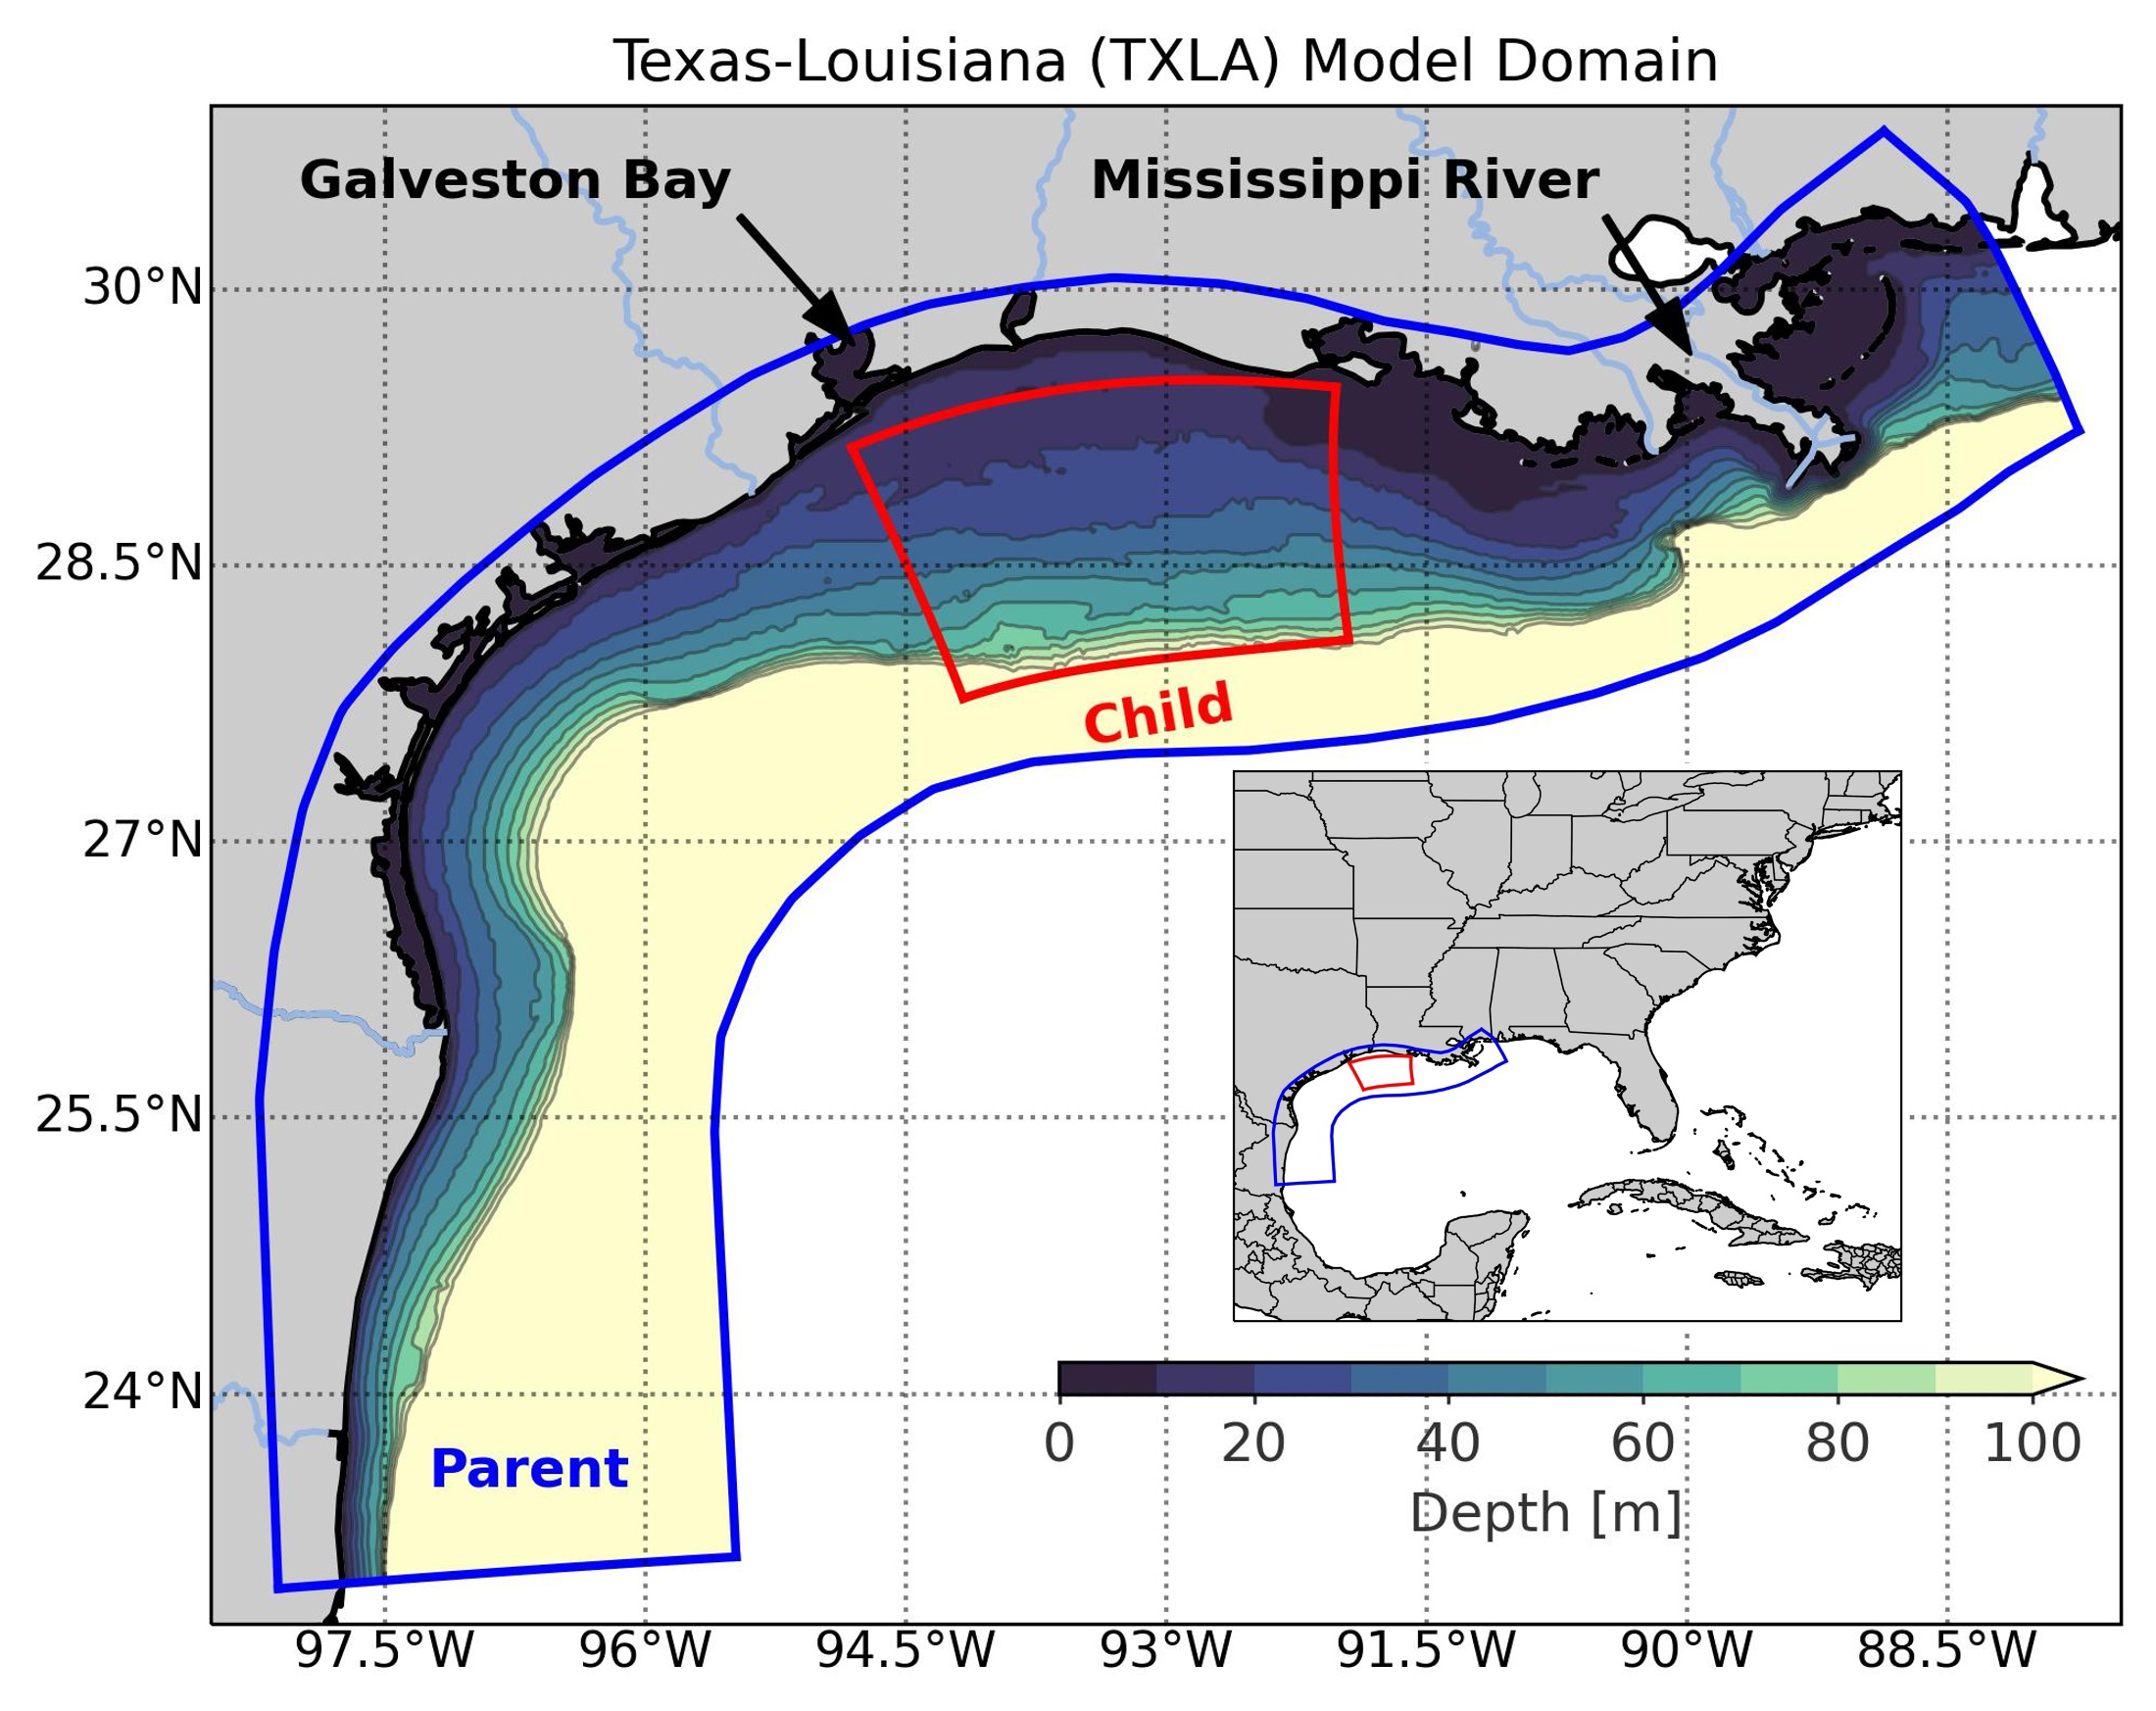
\includegraphics[width=0.9\textwidth]{figures/james_2023/Figure1_domain.jpg}}
    \caption{TXLA parent (coarse) and child (fine) model domain outlined with the blue and red lines, respectively. The colorbar displays the model bathymetry with a basemap located above the colorbar.}
    \label{fig:domain_overview}
\end{figure}

A third-order upwind scheme and a fourth-order centered scheme are used for momentum advection and Multidimensional Positive Definite Advection (MPDATA) is used for tracer advection \citep{Smolarkiewicz_1998}. The $k-\omega$ scheme is used for vertical mixing \citep{umlauf2003extending, Warner_2005} and horizontal mixing is parameterized along geopotential surfaces with constant horizontal viscosity (5.0 m$^2$s$^{-1}$) and diffusivity (1.0 m$^2$s$^{-1}$) values, both of which are scaled to the grid size. The model uses a baroclinic timestep of 75 s and a barotropic timestep of 1.875 s. The model provides hourly output and neglects tides because they are weak over the region \citep{DiMarco_1998}. The model is one-way nested into Global HYCOM Reanalysis to provide open boundary forcing and uses ERA-Interim datasets to provide surface forcing \citep{Dee_2011}. Additionally, the model uses streamflow data from nine rivers to provide freshwater forcing: Sabine, San Antonio, Trinity, Brazos, Calcasieu, Lavaca, Nueces, including the Mississippi and Atchafalaya, which provides the bulk of the discharge. The streamflow salinity is set to zero at all rivers and streamflow temperature is estimated using the bulk approach described by \citep{Stefan_1993}.

The nested model is configured to be two-way such that variables are exchanged across the open boundary. The bathymetry and vertical grid parameters of the child domain are the same as the parent's because the child domain was created from the parent domain. The bathymetry of the child domain was obtained by linearly interpolating the bathymetry of the parent domain. The ratio of the nesting is five to one, resulting in a mean horizontal resolution in the child model of 315 m. The surface fluxes, open boundaries and initial conditions were also obtained from the parent model by interpolating the parent model outputs to the child grid. By doing so, the models can reduce initialization shocks typically seen at the beginning of the simulation. A comparison between the parent and child grids along the open boundaries (i.e., contact points) showed that the fluxes in and out of the boundaries were internally conserved. 

The model has been used in several recent studies focusing on small-scale processes and dynamics in the nGoM \citep{Kobashi_2020,Qu_2021, Qu_2022_NIW, qu2022rapid, Xomchuk_2020}. For this study, we focus our analysis to the location of the child grid (Fig. \ref{fig:domain_overview}). The region is located west of the M/A river discharge points, which contribute to the generation of a baroclinic current over the shelf. The region is often saturated with eddies during summer (Fig. \ref{fig:surface_snapshots} e-f) due to formation of baroclinic instabilities \citep{Hetland_2017,Zhang_2012_numerical}. A diurnal land-sea breeze in near-resonance with the local inertial period forces near-inertial motions (e.g., waves and oscillations) that are perturbed by surface and river forcing \citep{zhang2009near}. The volume-integrated flow is strongly time dependent and serves as an excellent test case to investigate the accuracy of the offline methods in a realistic simulation. Previous studies focusing on submesoscale processes in the nGoM \citep{Barkan_2017,Luo_2016} have primarily focused east of the M/A discharge points in the aftermath of the 2010 \textit{Deepwater Horizon} oil spill. The wave-mean flow interactions in our study region can enhance mixing and lead to the rapid vertical exchange of biogeochemical tracers (e.g., oxygen), which becomes more pronounced as the horizontal resolution increases \citep{qu2022rapid}. We anticipate significant numerical mixing due to strong salinity gradients (Fig. \ref{fig:surface_snapshots} a-d), particularly near the northeastern boundary of the child domain where the Atchafalaya plume is more prevalent. 

\subsection{Simulation overview}

We performed two numerical simulations: one of the native TXLA model without nesting (hereinafter the ``coarse" simulation), and the second with nesting turned on (hereinafter the ``fine" simulation). Both simulations are analyzed from June 3 to July 13, 2010. Due to file corruption issues during the restart process of the fine simulation, we removed the following times (in UTC) from both the coarse and fine grid simulations when directly comparing the simulations: June 17 22:30 to June 18 19:30, June 19 14:30 to 19:30, and July 9 18:30. 

There are several notable mixing events driven by a combination of surface salt fluxes, wind stress, and freshwater input that otherwise contrast with periods of low physical mixing, allowing us to study numerical mixing under a variety of different environmental conditions. Over the inner shelf during the study period, contributions to density variations from variation in the temperature field are small relative to those from salinity variations. We focus our analysis to metrics that influence numerical mixing, in particular different metrics from the velocity gradient tensor normalized by the Coriolis parameter such as vertical relative vorticity $\zeta/f$, horizontal divergence $\delta/f$, horizontal strain rate $\alpha/f$, and the horizontal salinity gradient magnitude $|\nabla_H s|$. They are defined as:
\begin{equation}
    \zeta/f = \bigg(\frac{\partial v}{\partial x} - \frac{\partial u}{\partial y}\bigg)/f \quad ,
\end{equation}
\begin{equation}
    \delta/f = \bigg(\frac{\partial u}{\partial x} + \frac{\partial v}{\partial y}\bigg)/f \quad ,
\end{equation}
\begin{equation}
    \alpha/f = \sqrt{\bigg(\frac{\partial u}{\partial x} - \frac{\partial v}{\partial y}\bigg)^2+\bigg(\frac{\partial v}{\partial x} + \frac{\partial u}{\partial y}\bigg)^2}/f \quad ,
\end{equation}
\begin{equation}
    |\nabla_H s| = \sqrt{\bigg(\frac{\partial s}{\partial x} \bigg) ^2 + \bigg(\frac{\partial s}{\partial y} \bigg)^2} \quad .
\end{equation}
To isolate the effects of nesting on model processes, all variables discussed hereinafter from the coarse grid are subsetted offline to the location of the child grid and compared directly with the child grid of the fine simulation. Fig. \ref{fig:surface_snapshots} displays a sample of surface fields for the coarse and fine simulations of salinity, $|\nabla_H s|$, $\zeta/f$, $\delta/f$, and $\alpha/f$ during a time where numerous eddies are seen over the shelf. These eddies are considered to be submesoscale because they exhibit $\mathcal{O}(1)$ surface Rossby numbers, as approximated by $\zeta/f$ \citet{Barkan_2017, Kobashi_2020, McWilliams_2016}. The salinity of the fine simulation exhibits subtle differences near the northeastern boundary, however the effects of nesting are more striking in the vorticity. Several frontal eddies with anticyclonic cores and cyclonic filaments are resolved by both simulations. The cyclonic filaments are often associated with frontal convergence \citep{Kobashi_2020, qu2022rapid} and salinity gradients orders of magnitude stronger than those found in the anticyclonic cores where the the salinity is more homogeneous. The horizontal strain rate is enhanced throughout the fine simulation, which acts to sharpen the horizontal salinity gradients and enhance frontogenesis \citep{Hoskins_1972}.

\begin{figure} 
 \centerline{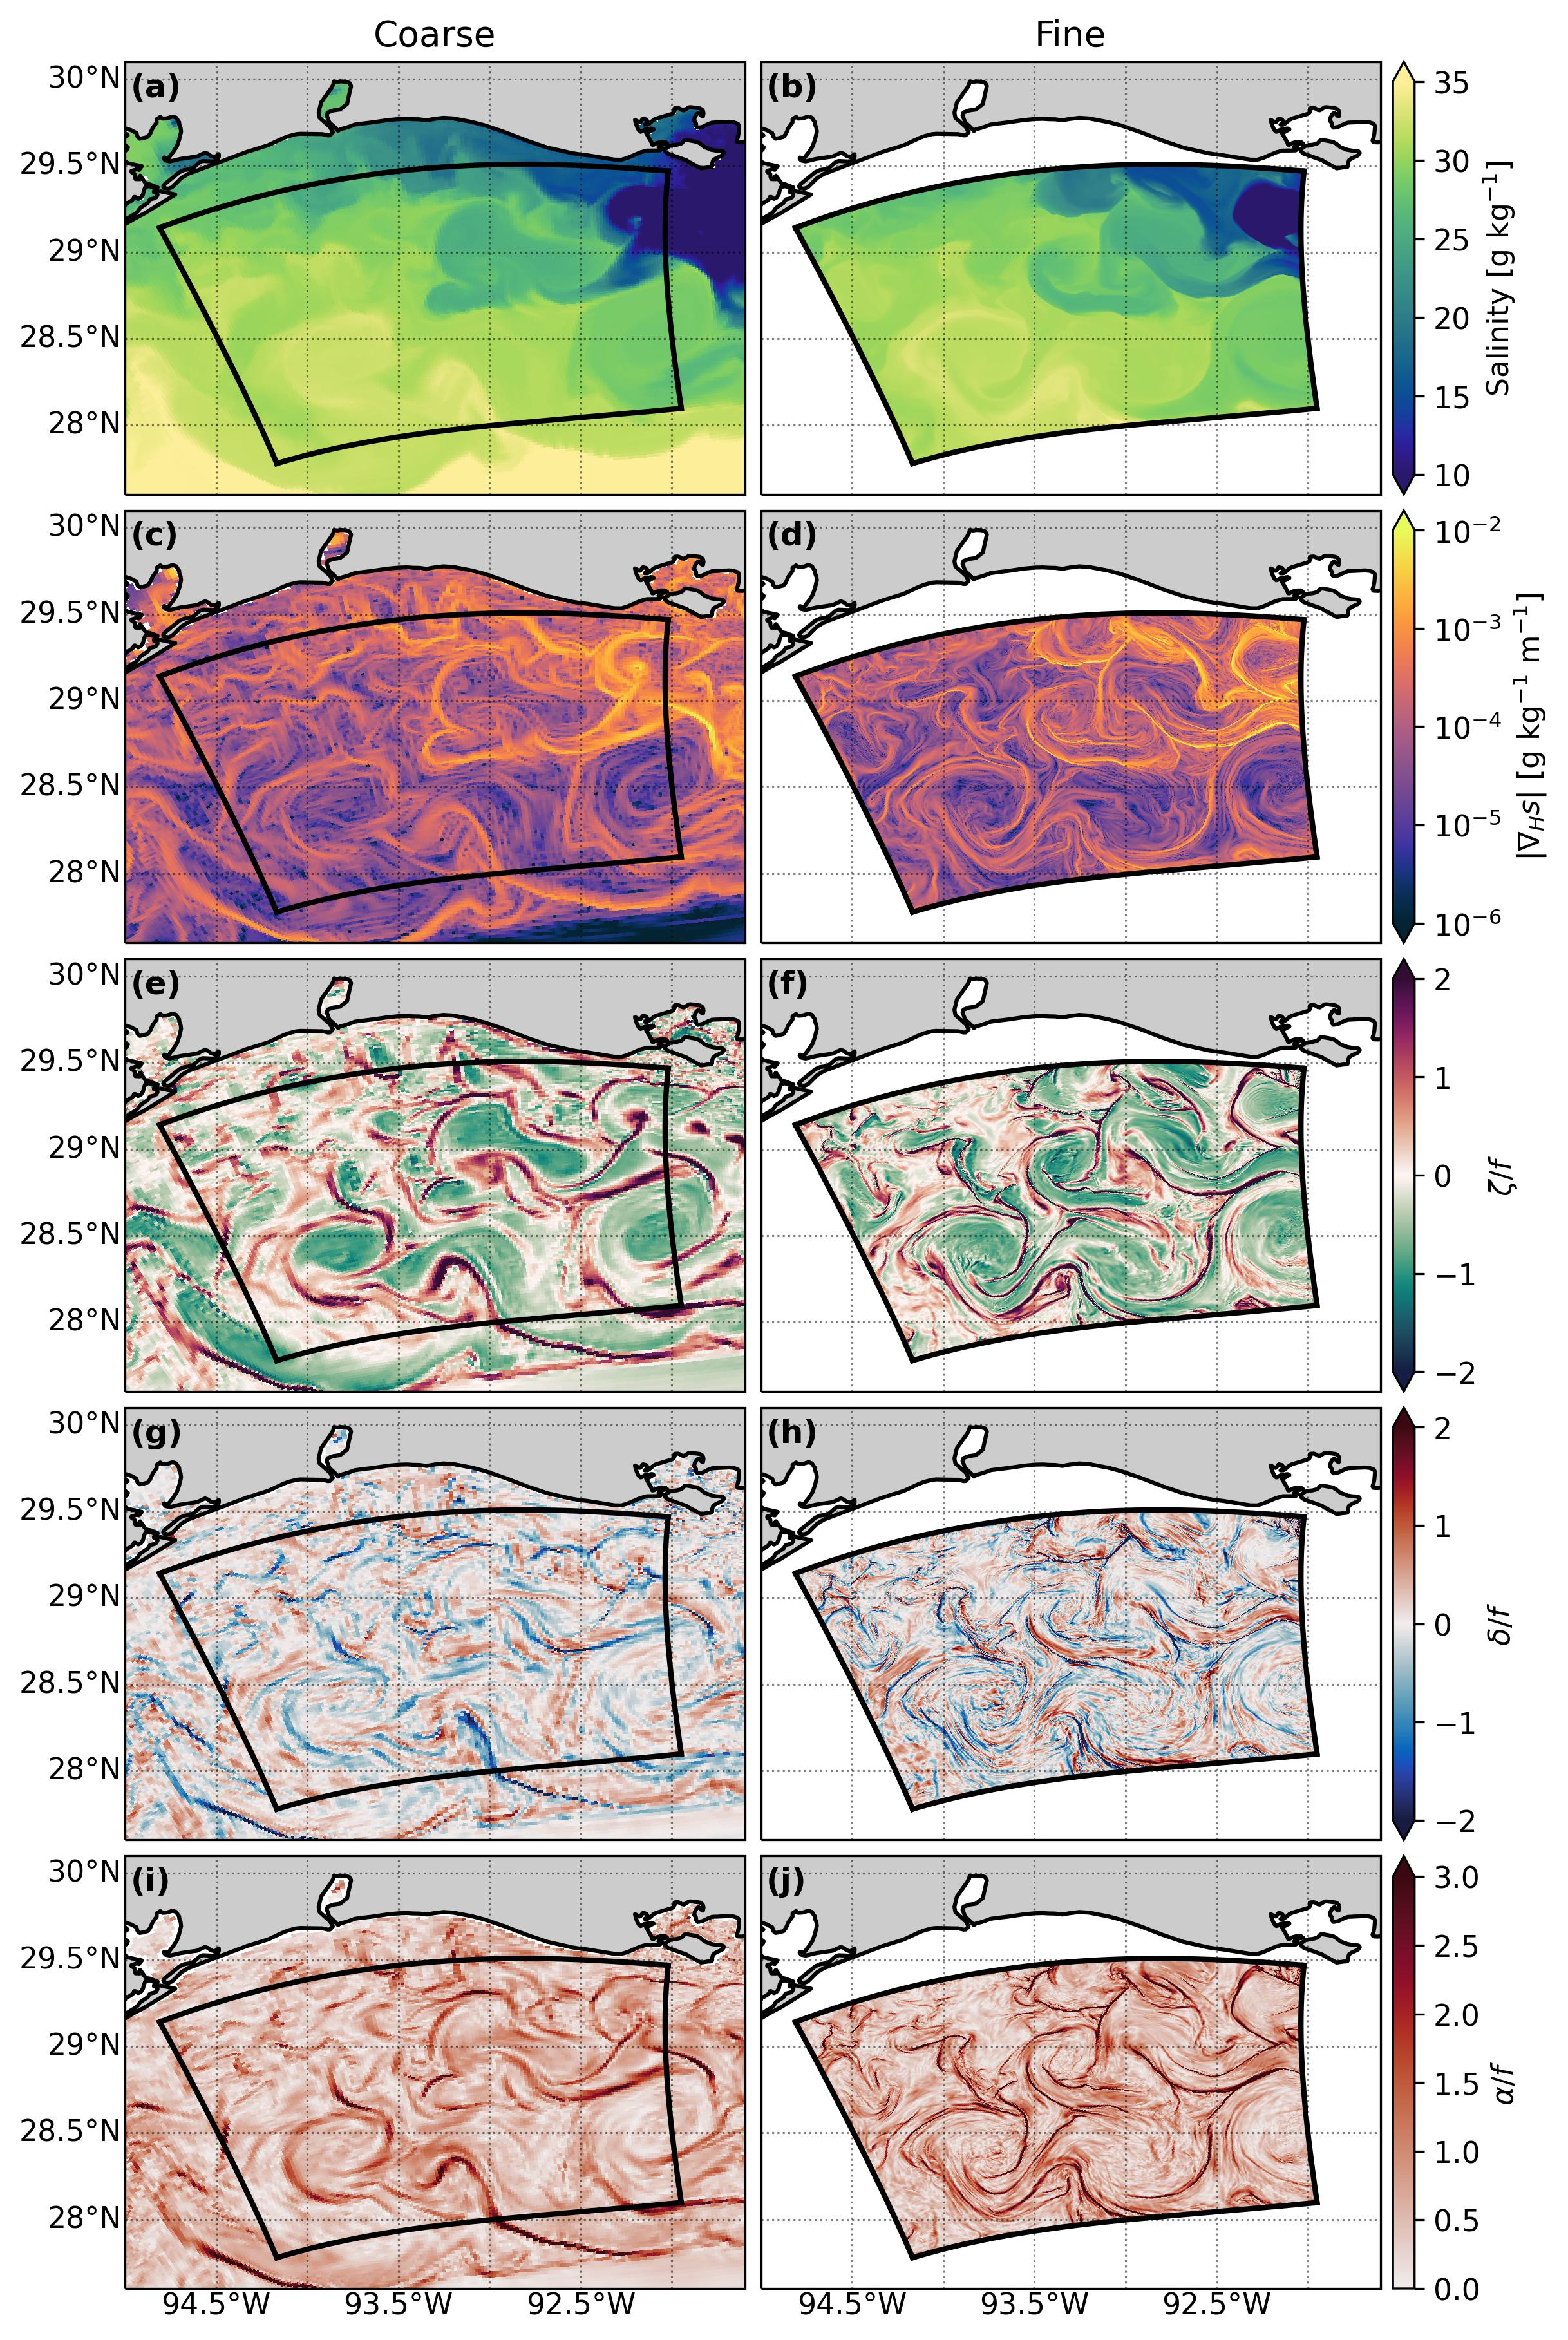
\includegraphics[width = 0.85\linewidth]{figures/james_2023/Figure2_snapshot.jpg}}
  \caption{Surface fields on June 20, 2010 12:30 UTC for the coarse (left column) and fine (right column) simulations of salinity (a-b), horizontal salinity gradient magnitude $|\nabla_H s|$ (c-d), relative vertical vorticity $\zeta/f$ (e-f), horizontal divergence $\delta/f$ (g-h), and horizontal strain rate $\alpha/f$ (i-j). Note that all velocity gradient tensor quantities are normalized by the Coriolis parameter $f$ and all variables are defined in text.}
  \label{fig:surface_snapshots}
\end{figure} 

To better understand the impacts of nesting on surface processes, Fig. \ref{fig:surface_pdfs} displays probability density functions (PDFs) of the various properties discussed above. Fig. \ref{fig:surface_pdfs} also displays the latter three quantities sorted by $\zeta/f>1$, which correspond to $\mathcal{O}(1)$ surface Rossby numbers associated with submesoscale fronts. The associated median and median-skewness of the velocity gradient tensor quantities and $|\nabla_H s|$ are shown in Table \ref{tab:1}. The relative vorticity is skewed cyclonically (positively) with a negative median for both simulations, with the median of the fine simulation decreasing by 159$\%$ and skewness increasing by 31\%. The divergence for both simulations have positive medians (i.e., divergence) and negative skewnesses, with the fine simulation increasing over 260\% and the skewness decreasing by 34\%. The strain for both models follows a $\chi$ distribution, consistent with the results of \citet{Shcherbina_2013}. The salinity gradient magnitude of the fine simulation has a slightly smaller median and skewness compared to the coarse simulation. When sorted by $\zeta/f>1$, the latter three quantities have significantly higher probabilities towards the tails of their distributions. This makes intuitive sense because the submesoscale fronts are associated with strong horizontal salinity gradients, elevated convergence/divergence, and elevated strain \citep{McWilliams_2016}. Interestingly, PDFs of $|\nabla_H s|$ remain essentially unchanged between the coarse and fine simulations, with slightly stronger gradients at the tail of the fine distribution, suggesting that changes to the velocity gradients do not necessarily result in similar changes to the salinity gradients. 

A possible explanation for the relatively unchanged salinity gradients in the nested model is due to the horizontal mixing scheme. ROMS scales grid-dependent horizontal diffusivities as
\begin{equation} \label{eq:kappa_H}
    \kappa_H = \frac{\kappa_{0}}{\max \sqrt{dA}}\sqrt{dA},
\end{equation}
where $\kappa_0$ is a prescribed background turbulent diffusivity (specified previously) and $dA$ is the lateral grid cell area. The maximum grid cell area is unique to each model grid, resulting in $\kappa_H$ being twice as large on average in the fine simulation compared to the coarse. As we will show in Section \ref{sec:results}, this increases the magnitude of the horizontal mixing and turbulent diffusion significantly, which may prevent the horizontal salinity gradients from sharpening as expected. 

\begin{figure}[ht] 
 \centerline{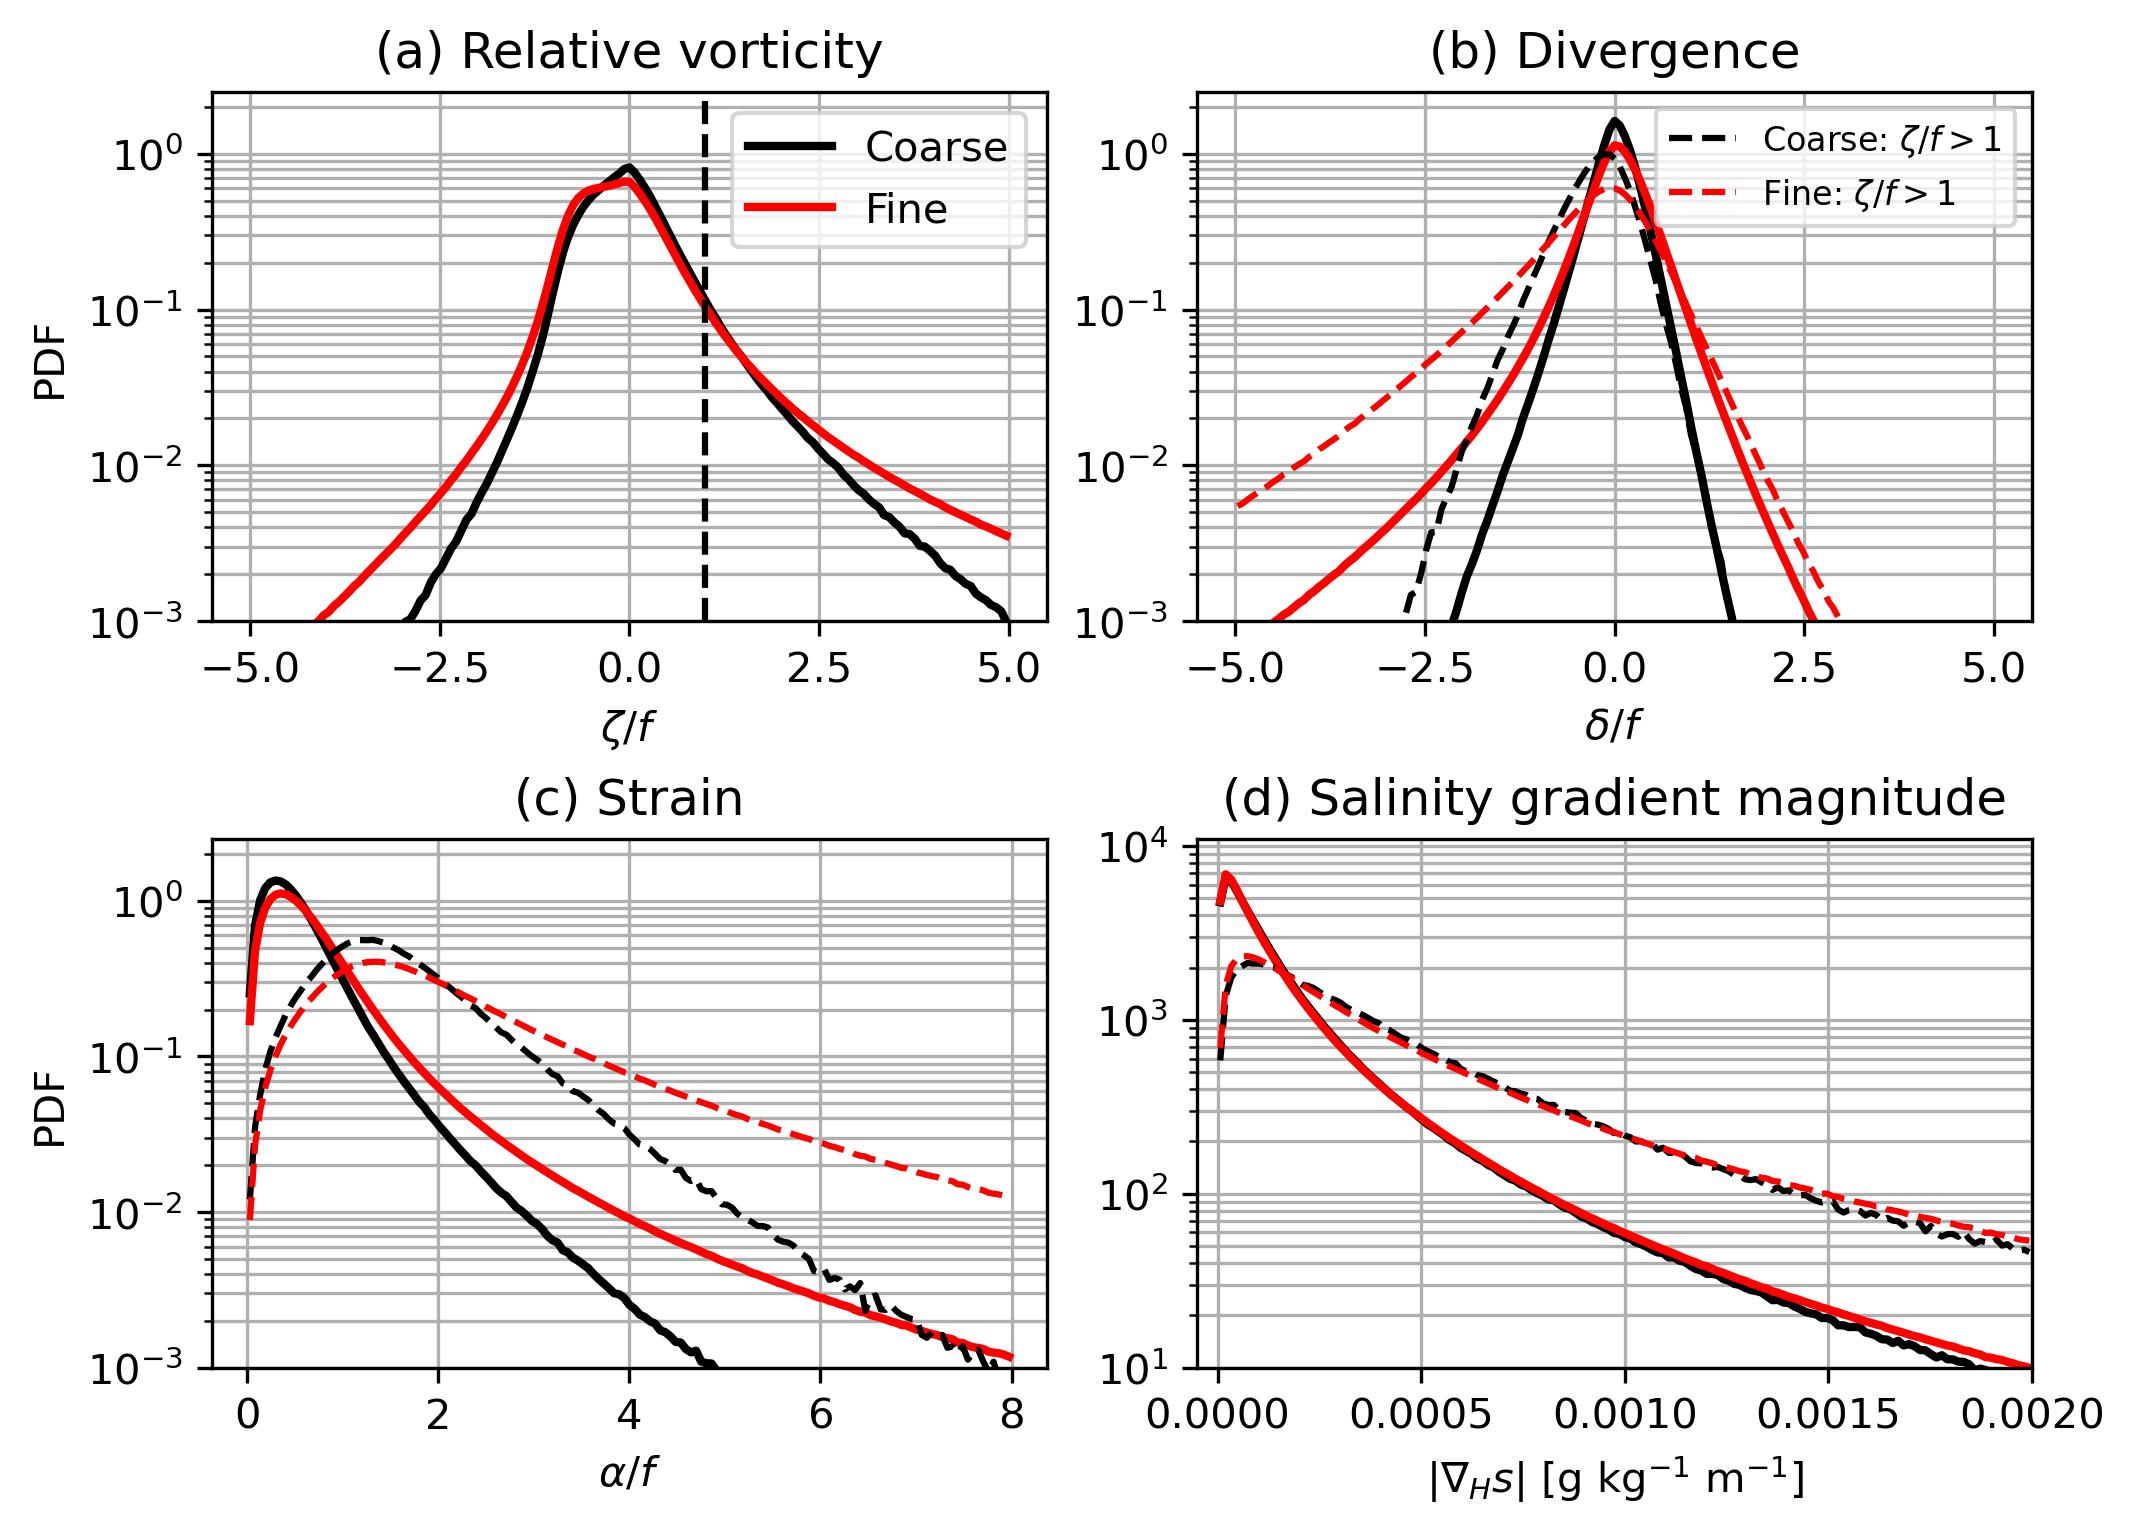
\includegraphics[width = \linewidth]{figures/james_2023/Figure3_surface_pdfs.jpg}}
  \caption{Probability density functions (PDFs) of surface $\zeta/f$ (a), $\delta/f$ (b), $\alpha/f$ (c), and $|\nabla_H s|$ (d) for the entire simulation period as defined in text. Dashed lines display $\delta/f$, $\alpha/f$, and $|\nabla_H s|$ sorted by $\zeta/f>1$ corresponding to the model fronts. The black dashed line in (a) demonstrates where $\zeta/f=1$. Each PDF was constructed discretely using 150 equal-spaced bins by first computing histograms and then normalized so the PDFs integrate to one.}
  \label{fig:surface_pdfs}
\end{figure}

 \begin{table}[h]
    \caption{Median and Pearson's median skewness for the surface and whole water column $\zeta/f$, $\delta/f$, $\alpha/f$, and $|\nabla_H s|$ for the coarse and fine simulations. Median quantities are denoted by an overline, and skewness quantities are denoted by a tilde. Median and skewness of the whole water column were computed by subsampling the coarse simulation every three $\xi, \eta \, (x,y)$ points and the fine simulation every 15 $\xi, \eta$ points. Note $|\nabla_H s|$ medians have units of g kg$^{-1}$ m$^{-1}$.}
    \centering
        \begin{tabular}{c c c c c c c c c}
        \hline
         Simulation & $\overline{\zeta/f}$ & $\widetilde{\zeta/f}$  & $\overline{\delta/f}$ &
         $\widetilde{\delta/f}$ &
         $\overline{\alpha/f}$  &
         $\widetilde{\alpha/f}$ & 
         $(\overline{|\nabla_H s|})*10^4$  &
         $\widetilde{|\nabla_H s|}$ \\
        \hline
         Coarse: Surf. & -0.054 & 0.296 & 0.009 & -0.154 & 0.470 & 0.757 & 1.000 & 0.926 \\
         Fine: Surf. & -0.140 & 0.399 & 0.0346 & -0.206 & 0.576 & 0.756 & 0.989 & 0.805 \\
         Coarse: Whole & -0.002 & 0.092 & 0.002 & -0.049 & 0.405 & 0.767 & 0.905 & 0.884 \\
         Fine: Whole &  -0.026 & 0.144 & 0.008 & -0.064 & 0.497 & 0.801 & 1.02 & 0.839 \\
        \hline
         \end{tabular} 
         \label{tab:1}
 \end{table}
 
Trends remain similar for the entire water column (Fig. \ref{fig:whole_pdfs}), however the distributions of $\zeta/f$ and $\delta/f$ are slightly more Gaussian. $\alpha/f$ still follows a $\chi$ distribution, but is significantly weaker relative to the surface distribution.  $|\nabla_H s|$ changes modestly compared to the velocity gradients, with the coarse simulation having slightly larger salinity gradients near the tails of the distribution. 

\begin{figure}[ht] 
 \centerline{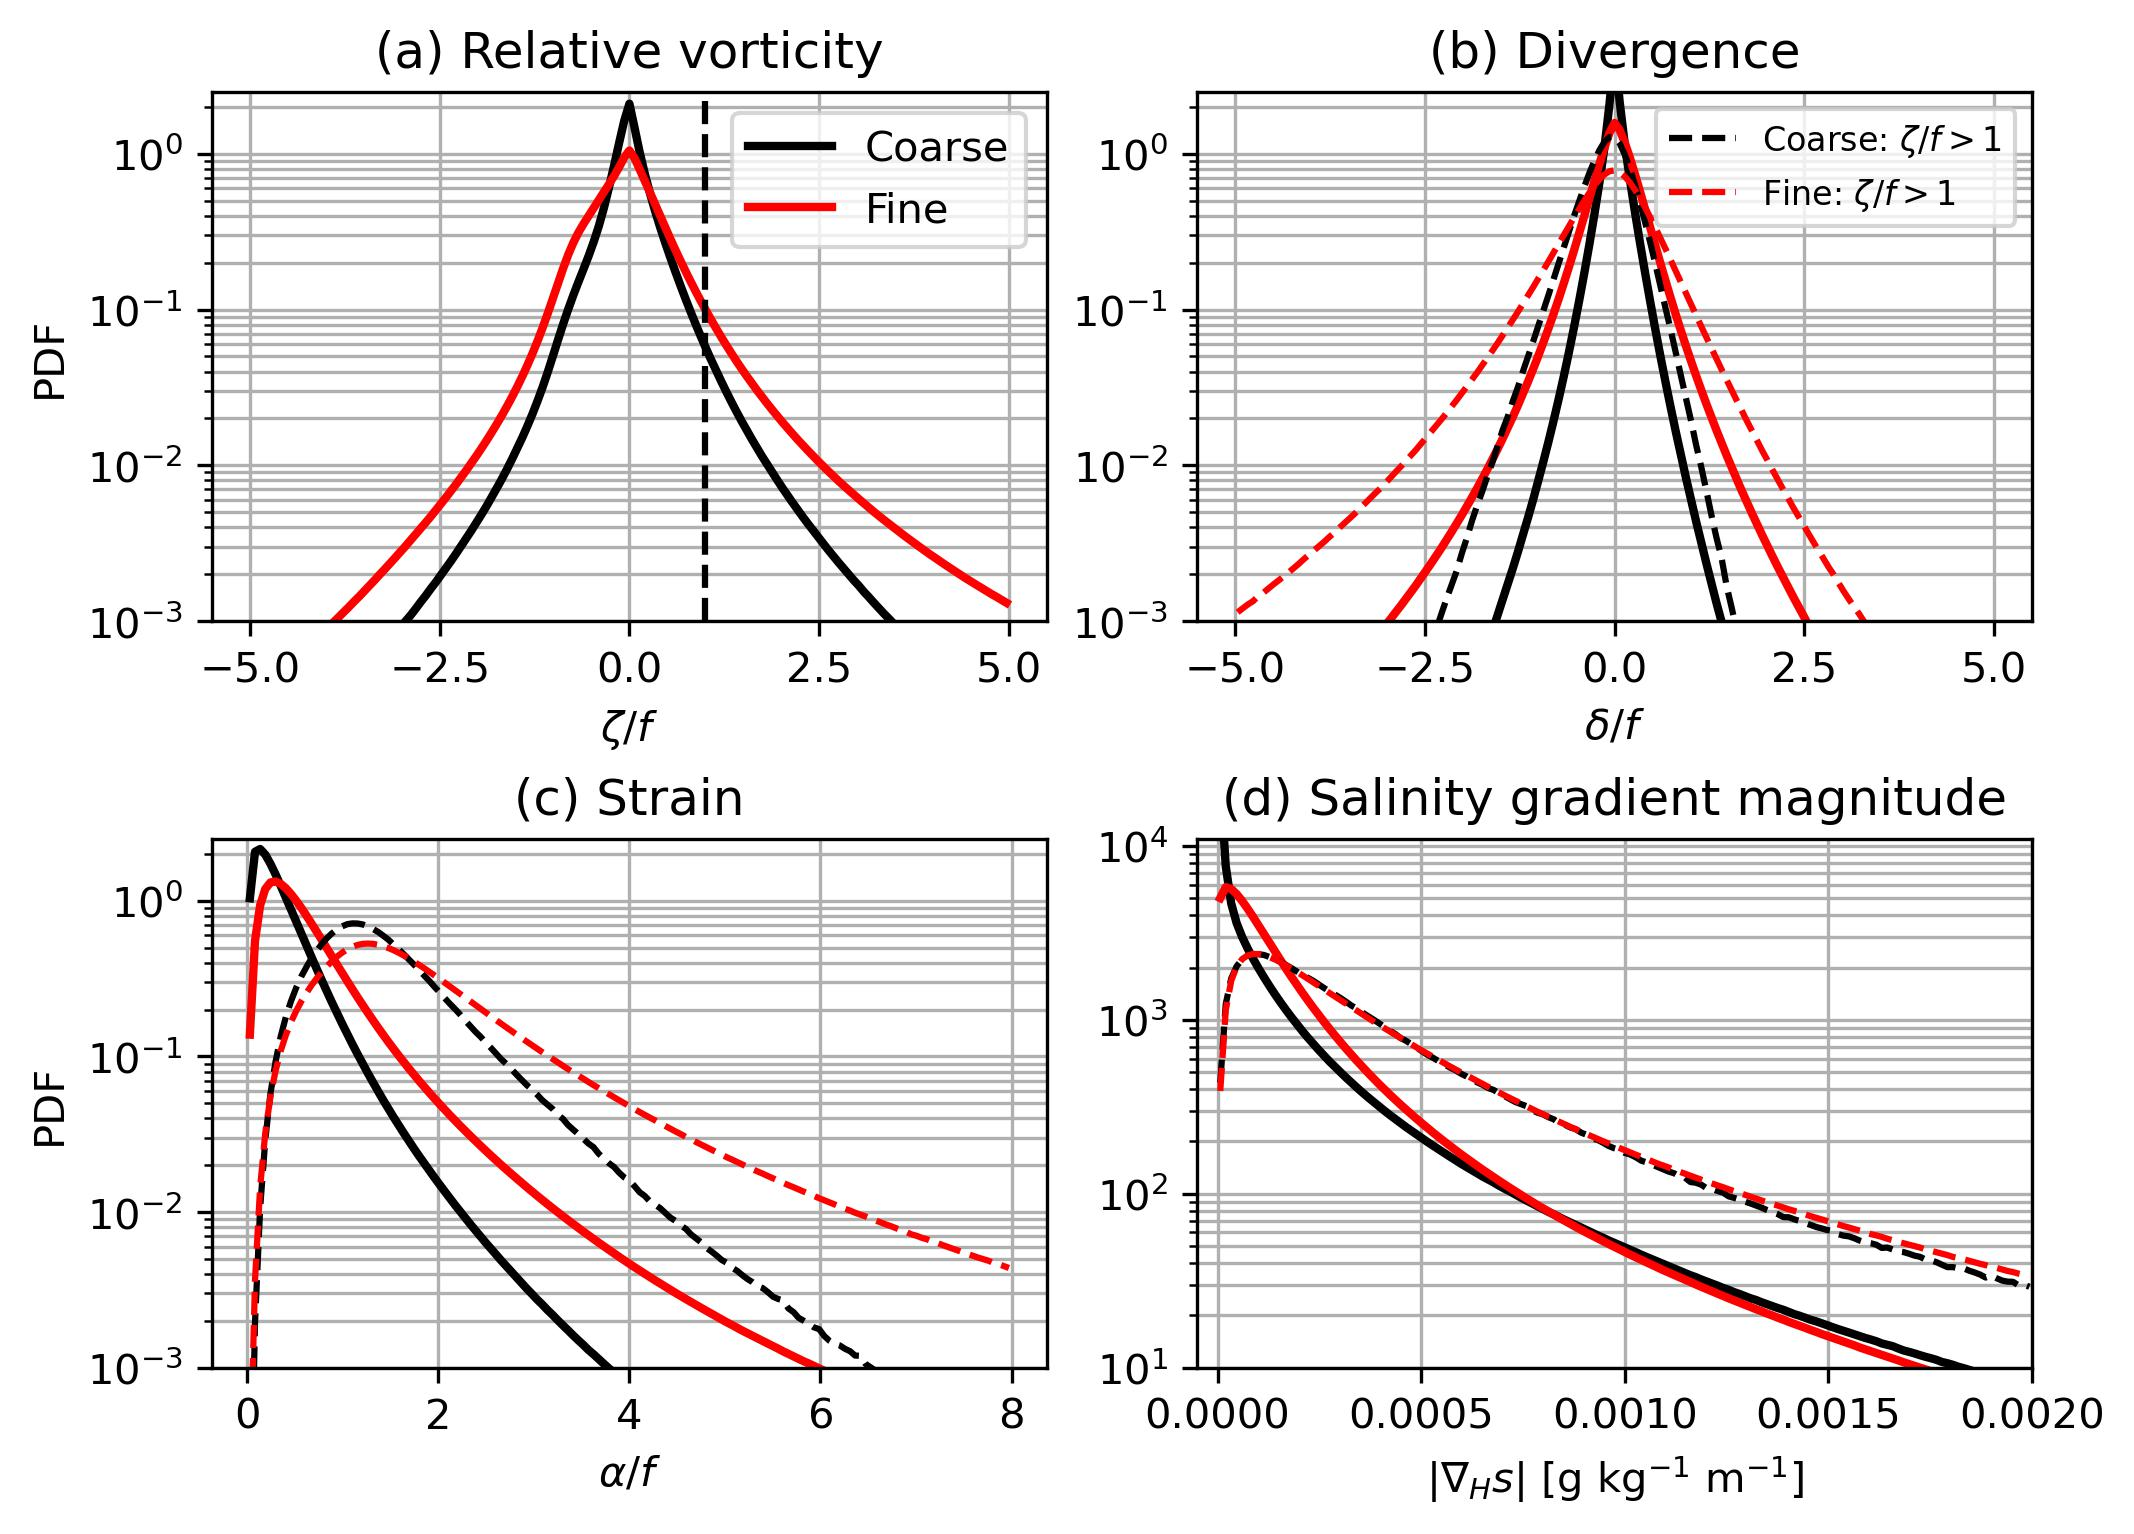
\includegraphics[width = \linewidth]{figures/james_2023/Figure4_whole_pdfs.jpg}}
  \caption{Same as Fig. \ref{fig:surface_pdfs}, but for the entire water column.}
  \label{fig:whole_pdfs}
\end{figure}

\subsection{Implementation of the online method for numerical mixing}

The online numerical mixing $\mathcal{M}_{num, on}$ is calculated locally following \citet{Burchard_2008}:   
\begin{equation}\label{Eq:mnum_online}
    \mathcal{M}_{num, on} = \frac{A\{ s^2 \}-\left(A \{s \} \right)^2}{\Delta t} \quad ,
\end{equation}
where $A$ is the advection operator (i.e., MPDATA) and $\Delta t$ is the model time step, which yields the numerical mixing in each grid cell. A discretized version of Eq. \ref{Eq:mnum_online} may be found in \citet{Burchard_2008}. $\mathcal{M}_{num, on}$ is computed using $s$ as the representative tracer instead of $s^{\prime}$ because $s^{\prime}$ requires calculating $\overline{s}$ for the location of the child grid during the model run. An analysis (not shown) of Eq. \ref{Eq:mnum_online} for a first order upwind scheme suggests that $\mathcal{M}_{num,on}$ should be identical whether $s$ or $s^\prime$ is used as the tracer. However, this is not necessarily the case for higher-order, nonlinear advection schemes that employ more sophisticated numerical algorithms. Therefore, it is unclear whether the online method should converge to $\mathcal{M}_{num, s^{\prime^2}}$ in addition to $\mathcal{M}_{num, s^2}$ if offline discretization errors are small. 

Although we will use the relative agreement between on- and offline methods as the basis to assess this, other sources of spurious mixing such as spurious convection due to high grid cell Reynolds numbers \citep{ilicak2016quantifying, Ilicak_2012}, cabbeling, and numerical diffusion may potentially contaminate both on- and offline methods. Generally, we do not expect these sources to be significant based on the results of \citet{Wang_2021}. We do not expect spurious convection to be significant because ROMS employs a third-order upstream advection scheme that enforces small grid-scale Reynolds numbers \citep{Ilicak_2012,shchepetkin2005regional}. Cabbeling is also not likely to be an issue, as work by \citet{barkan2017submesoscalepart2} slightly east of our study area suggested it is less significant in the M/A plume compared to other oceanic regions. However, we cannot say \textit{a priori} whether numerical diffusion will be significant. We will revisit these comments in Sections \ref{sec:results}-\ref{sec:discussion}. The numerical implementation of the offline method is shown in \ref{Appendix:offline_method}.

\section{Results} \label{sec:results}

\subsection{Spatial structure of the numerical and physical mixing}

To motivate our analysis of the physical and numerical mixing, Fig. \ref{fig:cross_section} displays cross-sections of $\mathcal{M}_{num, on}$ and $\chi^s$ split into horizontal and vertical components when a strong cross-shelf density gradient is generated by freshwater input for the coarse and fine simulations. A nearshore and offshore pycnocline are observed, where the nearshore pycnocline near 29$^\circ$N is associated with freshwater input from the Atchafalaya River and the offshore near pycnocline is associated with freshwater input from the Mississippi River \citep{Kobashi_2020}. The numerical mixing, although noisy, is approximately 2.75 times larger when averaged over the cross section in the coarse simulation compared to the physical mixing and may be orders of magnitude larger locally. The negative mixing is due to the anti-diffusive properties of MPDATA, which acts to reduce the total mixing but does not have a physical interpretation. The numerical mixing is concentrated primarily where the isopycnals are pinched in the pycnoclines, generally corresponding to strong horizontal salinity gradients. Stronger salinity gradients are located shoreward of 29.25$^{\circ}$N, however the numerical mixing is small relative to the offshore pycnocline, likely due to increased grid resolution. Previous studies have shown that numerical mixing is related to the horizontal salinity gradients \citep{hofmeister2011realistic, Kalra_2019, Klingbeil_2014,Wang_2021} and we investigate this more in Section \ref{sec:discussion}.

\begin{figure}
 \centerline{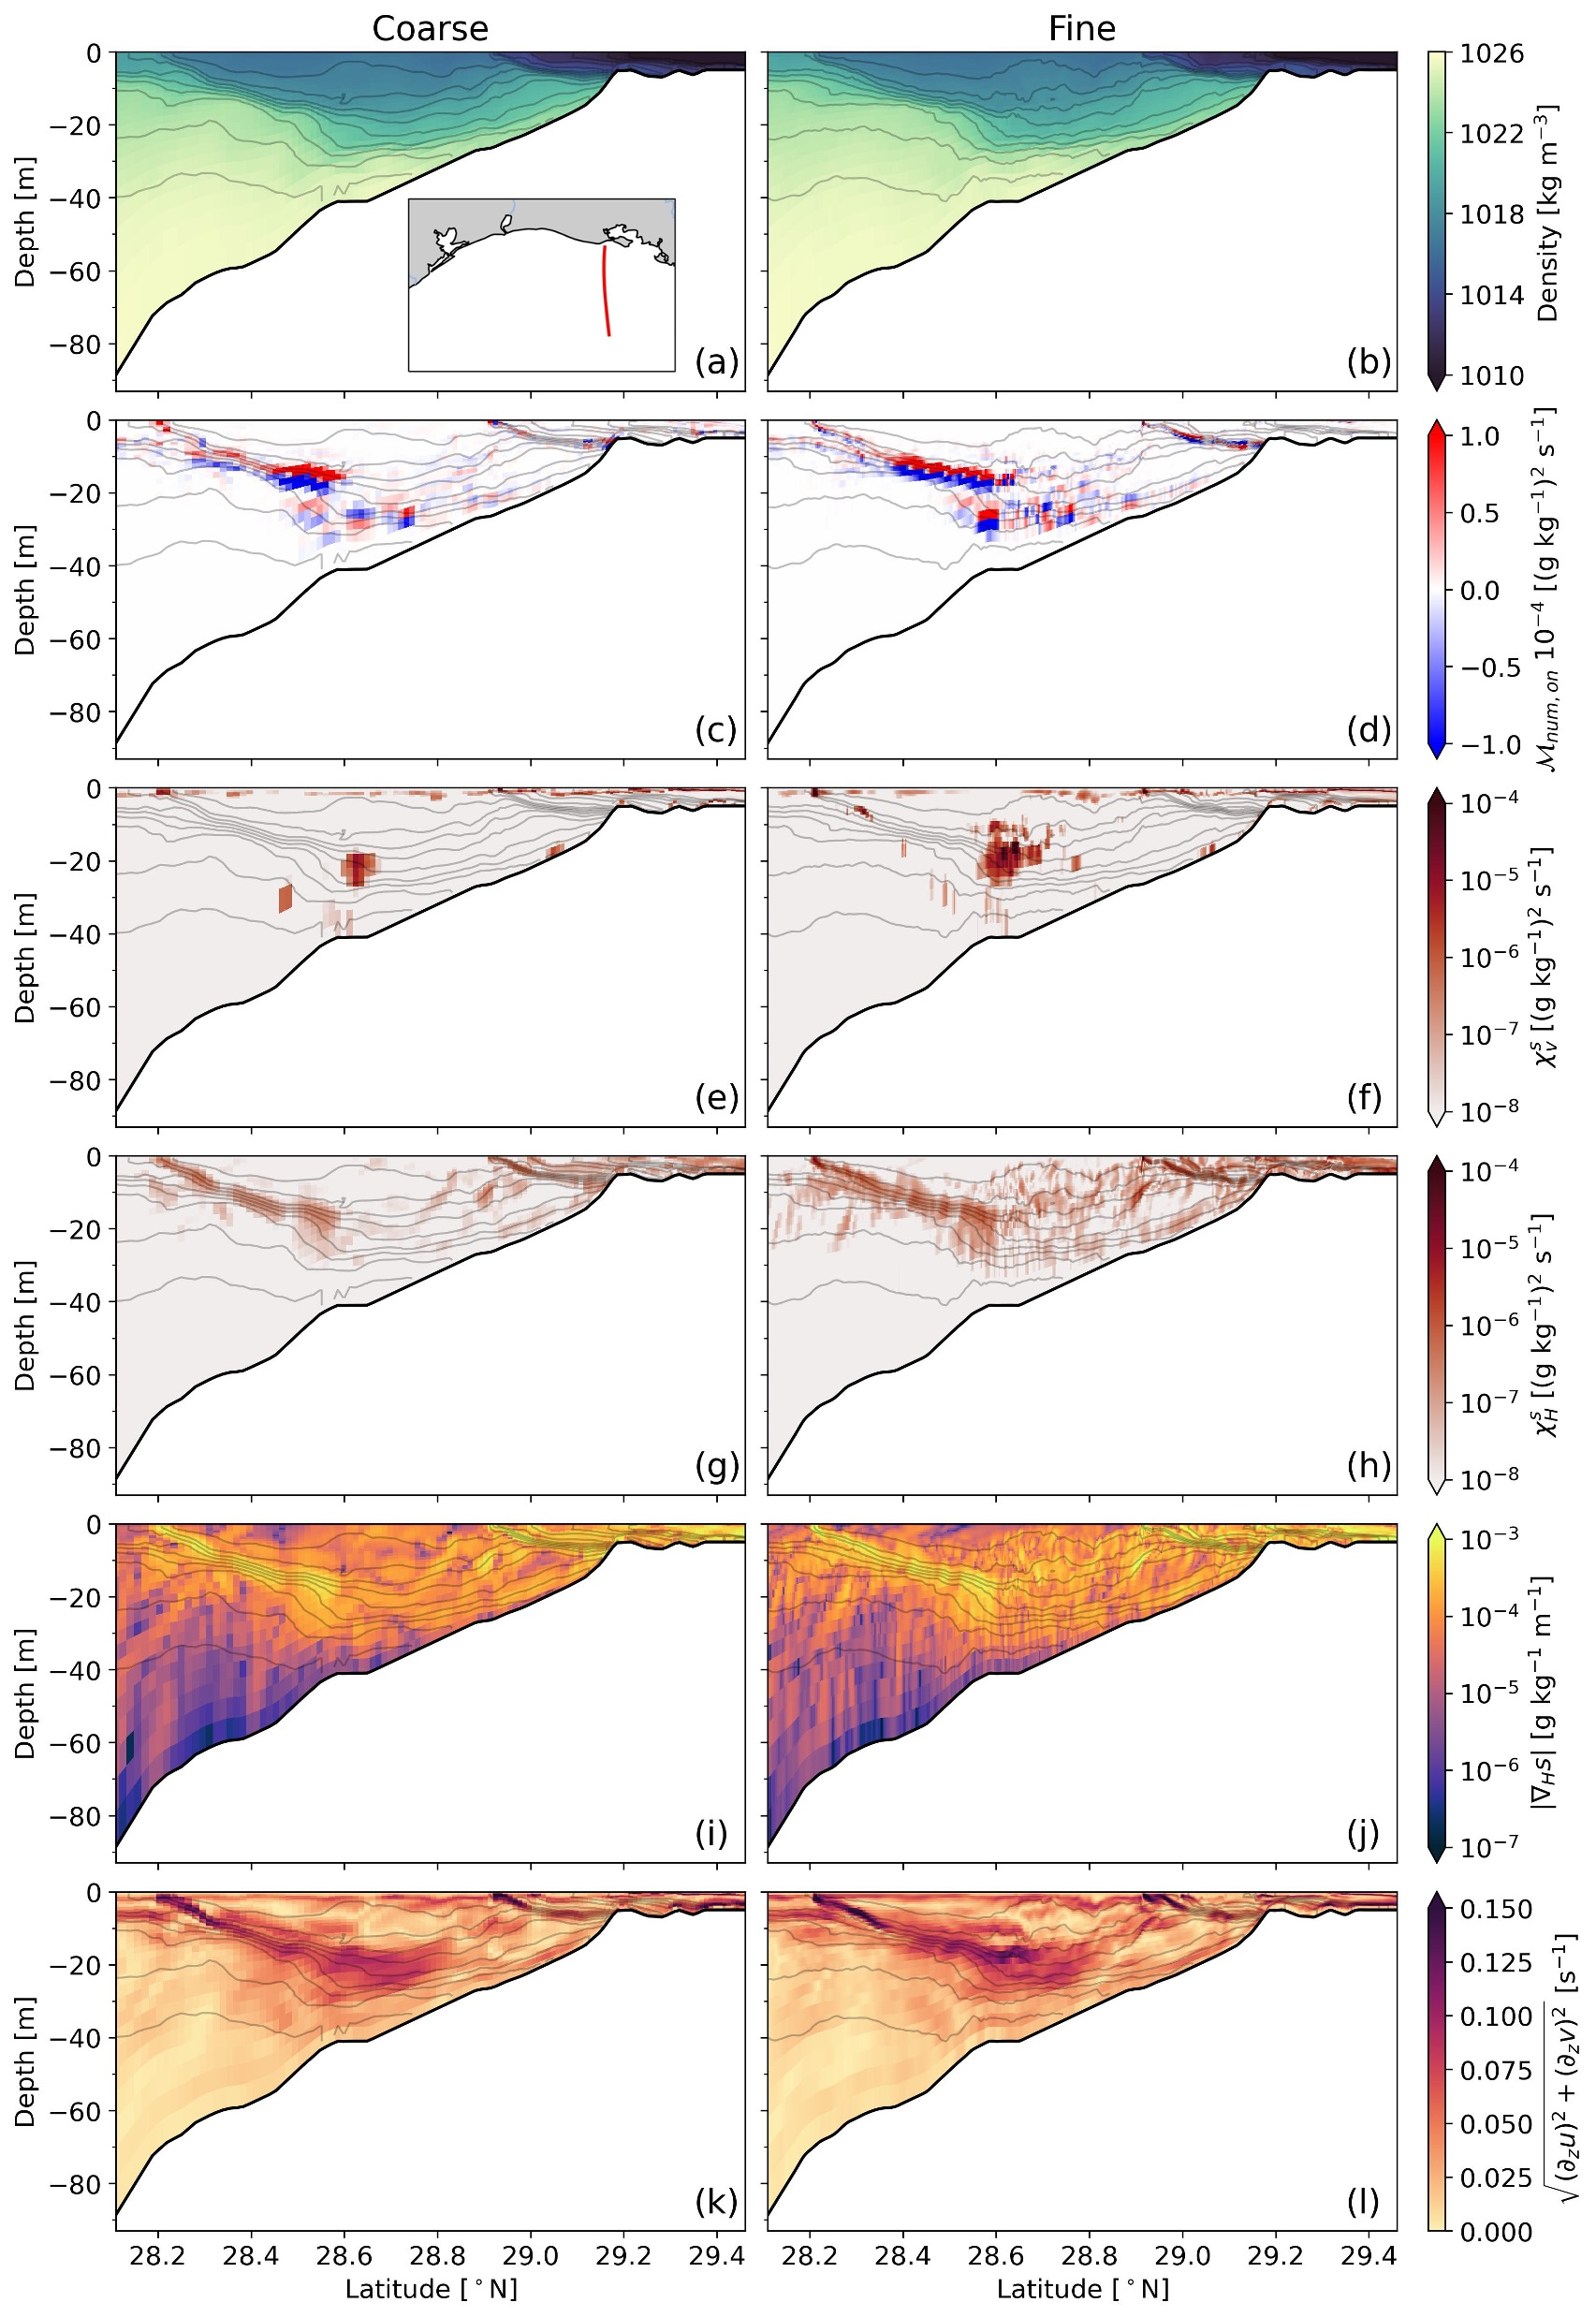
\includegraphics[width = 0.85\linewidth]{figures/james_2023/Figure5_cross_section.jpg}}
  \caption{Cross-sections for the coarse (left) and fine (right) simulations examining mixing and related properties where a strong cross-shelf density gradient is present on June 8, 2010 00:30 UTC. Density (a-b), $\mathcal{M}_{num, on}$ (c-d), $\chi_v^s$ (e-f), $\chi_H^s$ (g-h), $|\nabla_H s|$ (i-j), and magnitude of vertical shear $\sqrt{(\partial_z u)^2+(\partial_z v)^2}$ (k-l). Isopycnals are displayed with gray lines every kg m$^{-3}$ for the range shown in the colorbar. Note that the numerical mixing is on a linear scale and the physical mixing is on a log scale.}
  \label{fig:cross_section}
\end{figure}

The physical mixing exhibits different spatial trends when broken into horizontal ($\chi_H^s$) and vertical $\chi_v^s$ components. This is due to two reasons: different parameterizations for the horizontal and vertical turbulent diffusivities and different distributions of the horizontal and vertical salinity gradients. $\chi_v^s$ is concentrated at the surface and in the middle of cross-section. The areas of high physical mixing roughly correspond to where the vertical shear and turbulent diffusivity are strong (and large vertical velocity variance). Similar to the numerical mixing, $\chi_H^s$ is strongly correlated with $|\nabla_H s|$ and comprises 9.1$\%$ of the total physical mixing ($\chi_H^s+\chi_v^s$) when averaged over the cross section. 

Model nesting produces several notable differences, although the general trends remain the same. There are several locations where the numerical mixing in the fine simulation is stronger than the coarse simulation. The physical mixing averaged over the cross-section in the fine simulation is larger than the coarse simulation, with $\chi_H^s$ now comprising 24$\%$ of the total physical mixing. As discussed in Section 3, this is primarily due to an increase in the magnitude of $\kappa_H$ in the fine simulation. The spatially-averaged numerical mixing decreases by $51$\%, with the mean numerical mixing being positive for both simulations. In this particular cross-section, the decrease in average numerical mixing appears to be due to a more symmetric distribution of positive and negative values, which is evident in probability density functions and estimates of skewness over the cross-section. Eq. \ref{Eq:mnum_online} is limited in this application because it does not separate the horizontal and vertical contributions of tracer advection to numerical mixing. Horizontal and vertical tracer advection are often computed with different subroutines in ocean models, which could allow $\mathcal{M}_{num, on}$ to be decomposed into components. Such a decomposition could be used to assess whether refinement of the horizontal or vertical grid resolution is required to reduce numerical mixing.

To examine the broader spatial variability, Fig. \ref{fig:depth_integrated} displays depth- and time-integrated $\chi^s$ and $\mathcal{M}_{num, on}$, the ratio of integrated $\chi_H^s$ to $\chi_v^s$, and the ratio of integrated $\mathcal{M}_{num, on}$ to $\chi^s$. Both $\chi_v^s$ and $\mathcal{M}_{num, on}$ are strongest near the northeastern boundary due to a large influx of brackish water from the M/A river plume. $\chi_H^s$ is more significant near the southwestern boundary. This is unsurprising because the vertical salinity gradients will be weaker relative to the horizontal further offshore where the plume stratification is weaker (in contrast to the northeastern boundary). The integrated $\mathcal{M}_{num, on}$ in the coarse simulation is significantly noisier, with a small patch of negative values concentrated near the northeastern boundary. As a consequence, this will decrease the total mixing and may spuriously alter the timescales of mixing processes associated with submesoscale fronts, although more analysis is needed to confirm this. The integrated $\mathcal{M}_{num, on}$ exceeds $\chi^s$ for a significant portion of the domain in the coarse simulation, with the greatest discrepancy occurring near the southwestern boundary where $\chi^s$ is weaker. 

There is a marked enhancement of integrated $\chi^s$ in the fine simulation. This is especially true for the ratio of $\chi_H^s$ to $\chi_v^s$. As discussed previously, we believe this is due to an increase in $\kappa_H$ of the fine simulation. A newly resolved patch of $\chi^s$ in the fine simulation spanning almost half the latitudinal extent of the domain is seen east of $93^{\circ}$W. $\mathcal{M}_{num, on}$ is reduced throughout the domain of the fine simulation. Additionally, the ratio of $\mathcal{M}_{num, on}$ to $\chi^s$ substantially decreases in the fine simulation, with the numerical mixing exceeding the physical mixing in several patches near the southwestern boundary.

\begin{figure}
 \centerline{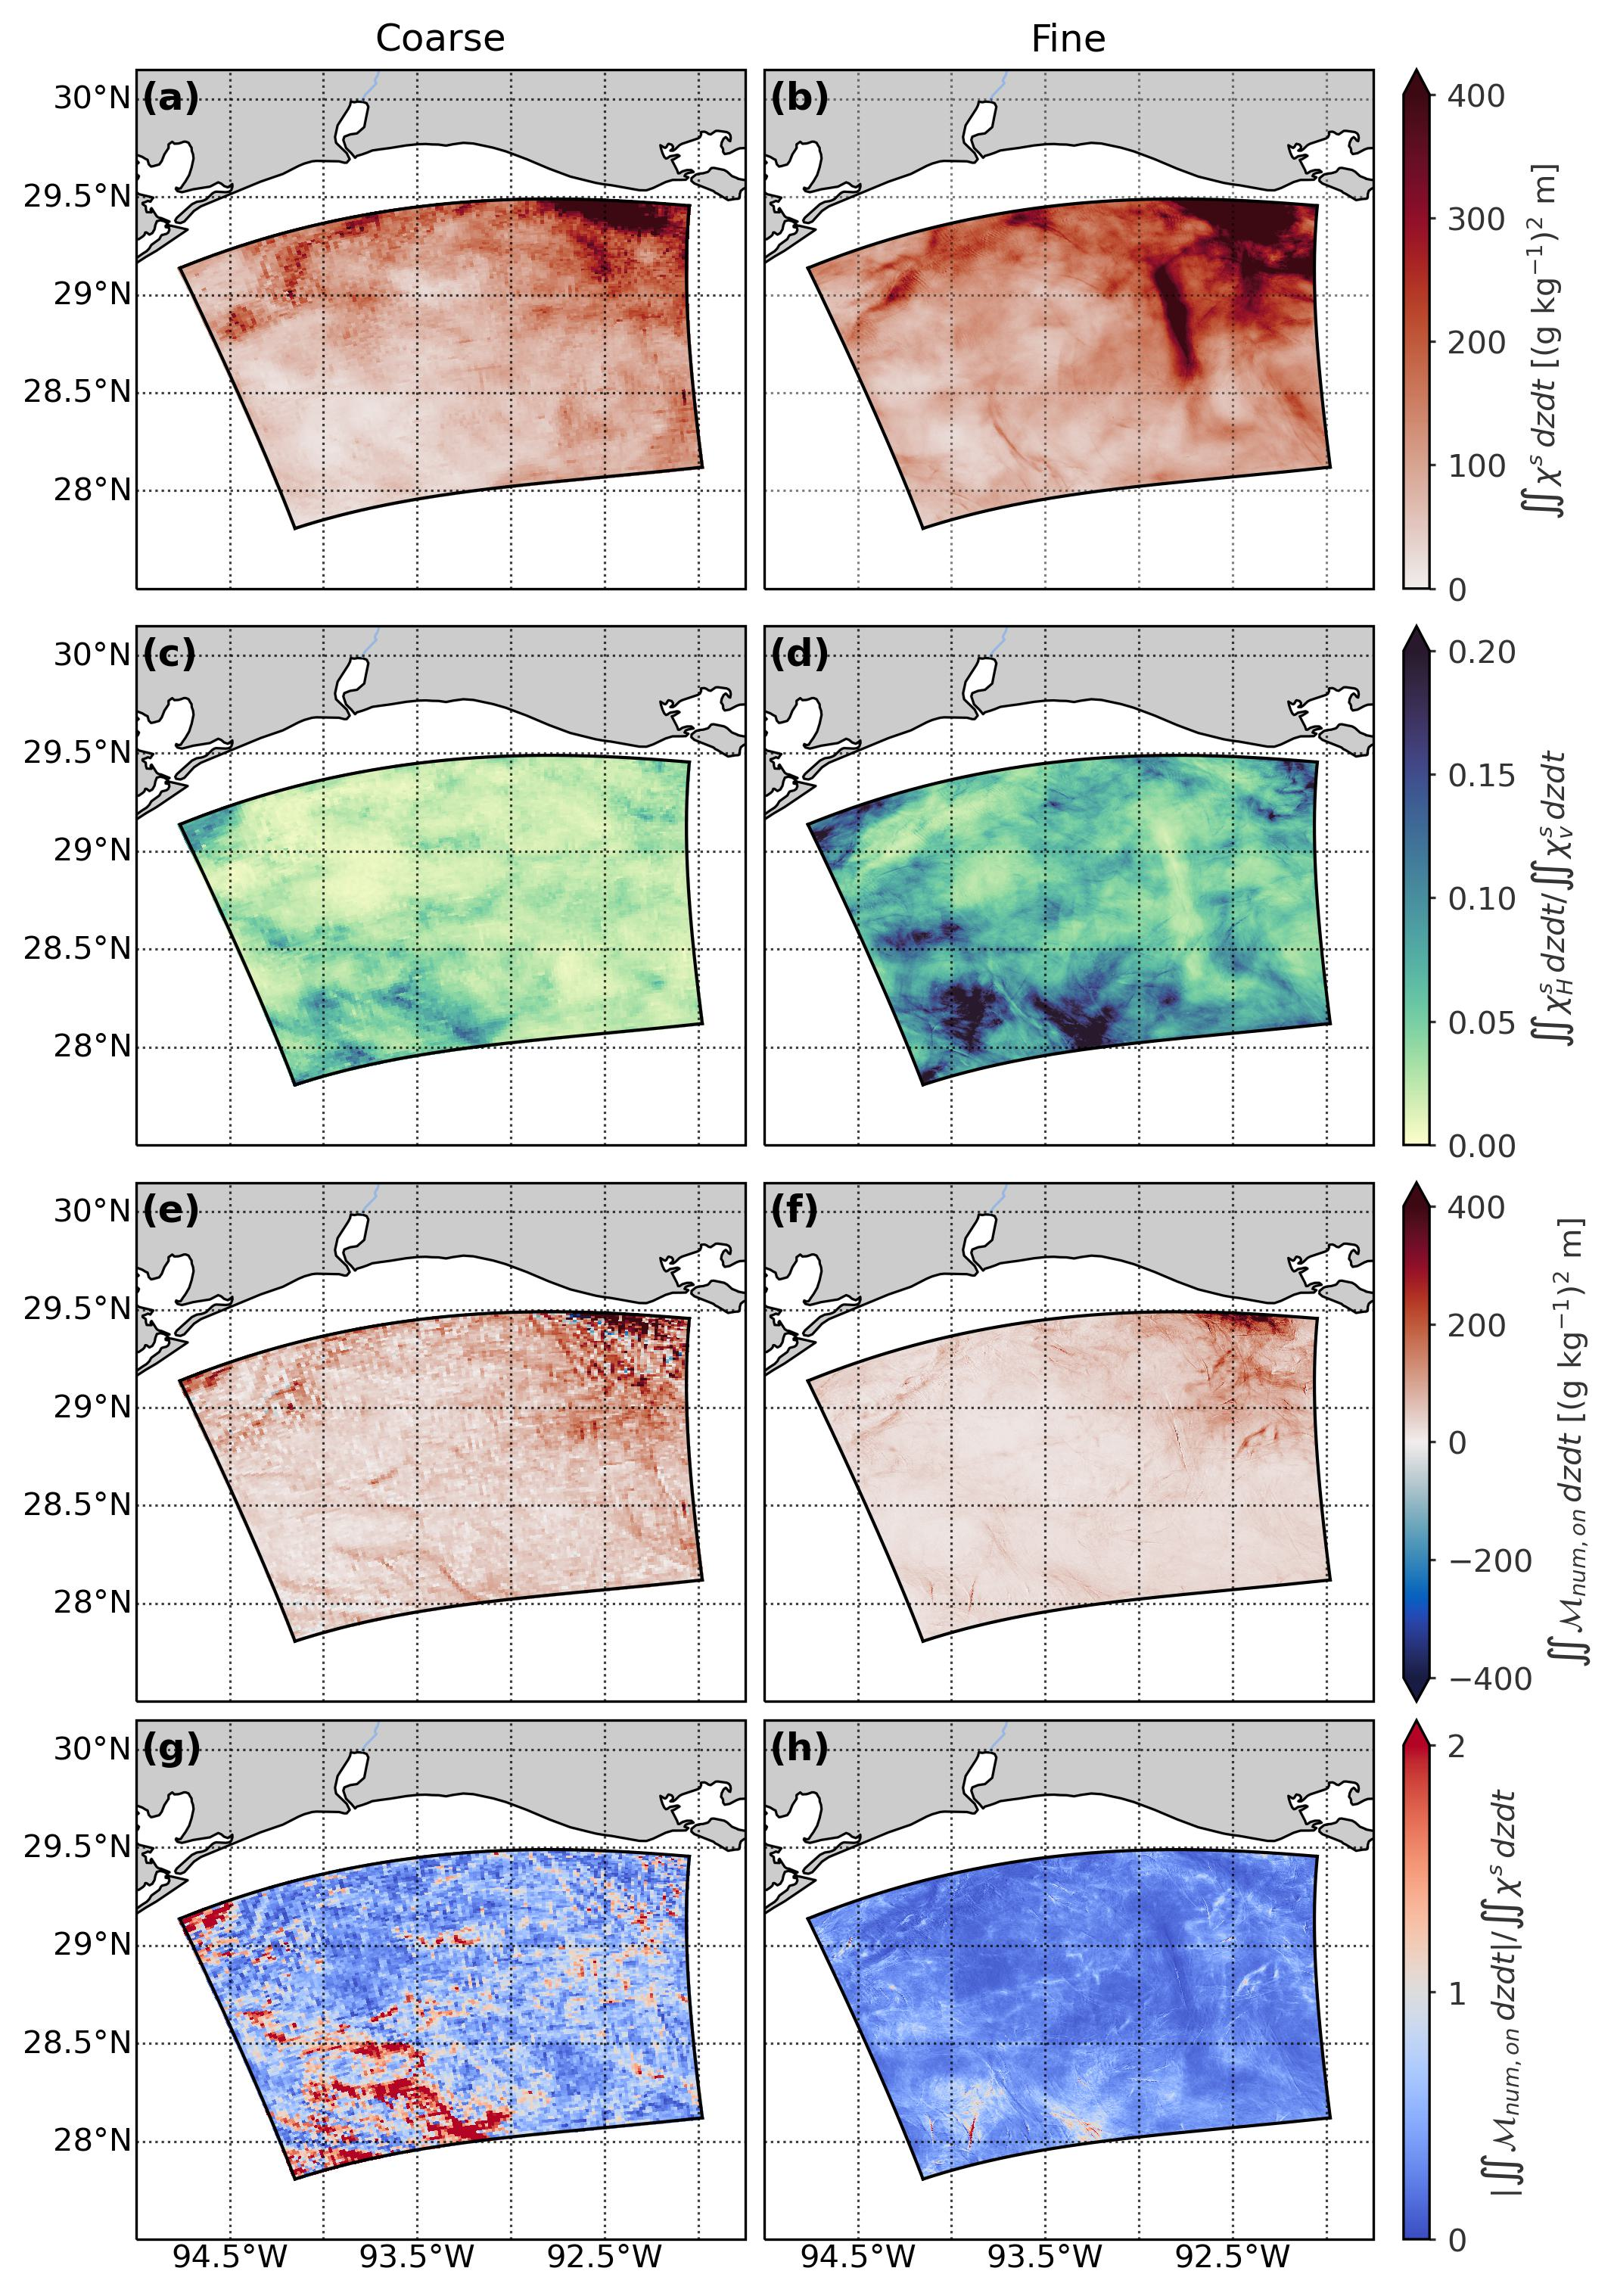
\includegraphics[width = 0.85\linewidth]{figures/james_2023/Figure6_dzdt_int.jpg}}
  \caption{Various depth and time-integrated mixing quantities for the coarse and fine simulations. Depth- and time-integrated total physical mixing $\chi^s$ (a-b). Ratio of depth- and time-integrated $\chi_H^s$ to $\chi_v^s$ (c-d), where bluer colors indicate more horizontal physical mixing and greener colors indicate less horizontal physical mixing. Depth- and time-integrated $\mathcal{M}_{num, on}$ (e-f). Ratio of depth- and time-integrated $\mathcal{M}_{num,on}$ and $\chi^s$ (g-h), where red colors indicate more numerical mixing and blue colors indicate less numerical mixing.}
  \label{fig:depth_integrated}
\end{figure}

\subsection{Temporal variability}

Here, we explore the volume-integrated $s^2$ and $s^{\prime^2}$ budgets and compare the accuracy of the numerical mixing estimated from the $s^{\prime^2}$ budget to the online method. Fig. \ref{fig:budget_comparison} shows a time series for the coarse simulation of surface wind forcing, the terms in Eqs. \ref{eq:salt2_vint} and \ref{eq:svar_int}, and a comparison between the different methods for quantifying volume-integrated numerical mixing. All wind forcing was spatially averaged over the location of the child grid. The land-sea breeze can generally be seen throughout the simulation, with several exceptions (e.g., June 30 and July 7) due to transient wind events such as storms. 

\begin{figure}
 \centerline{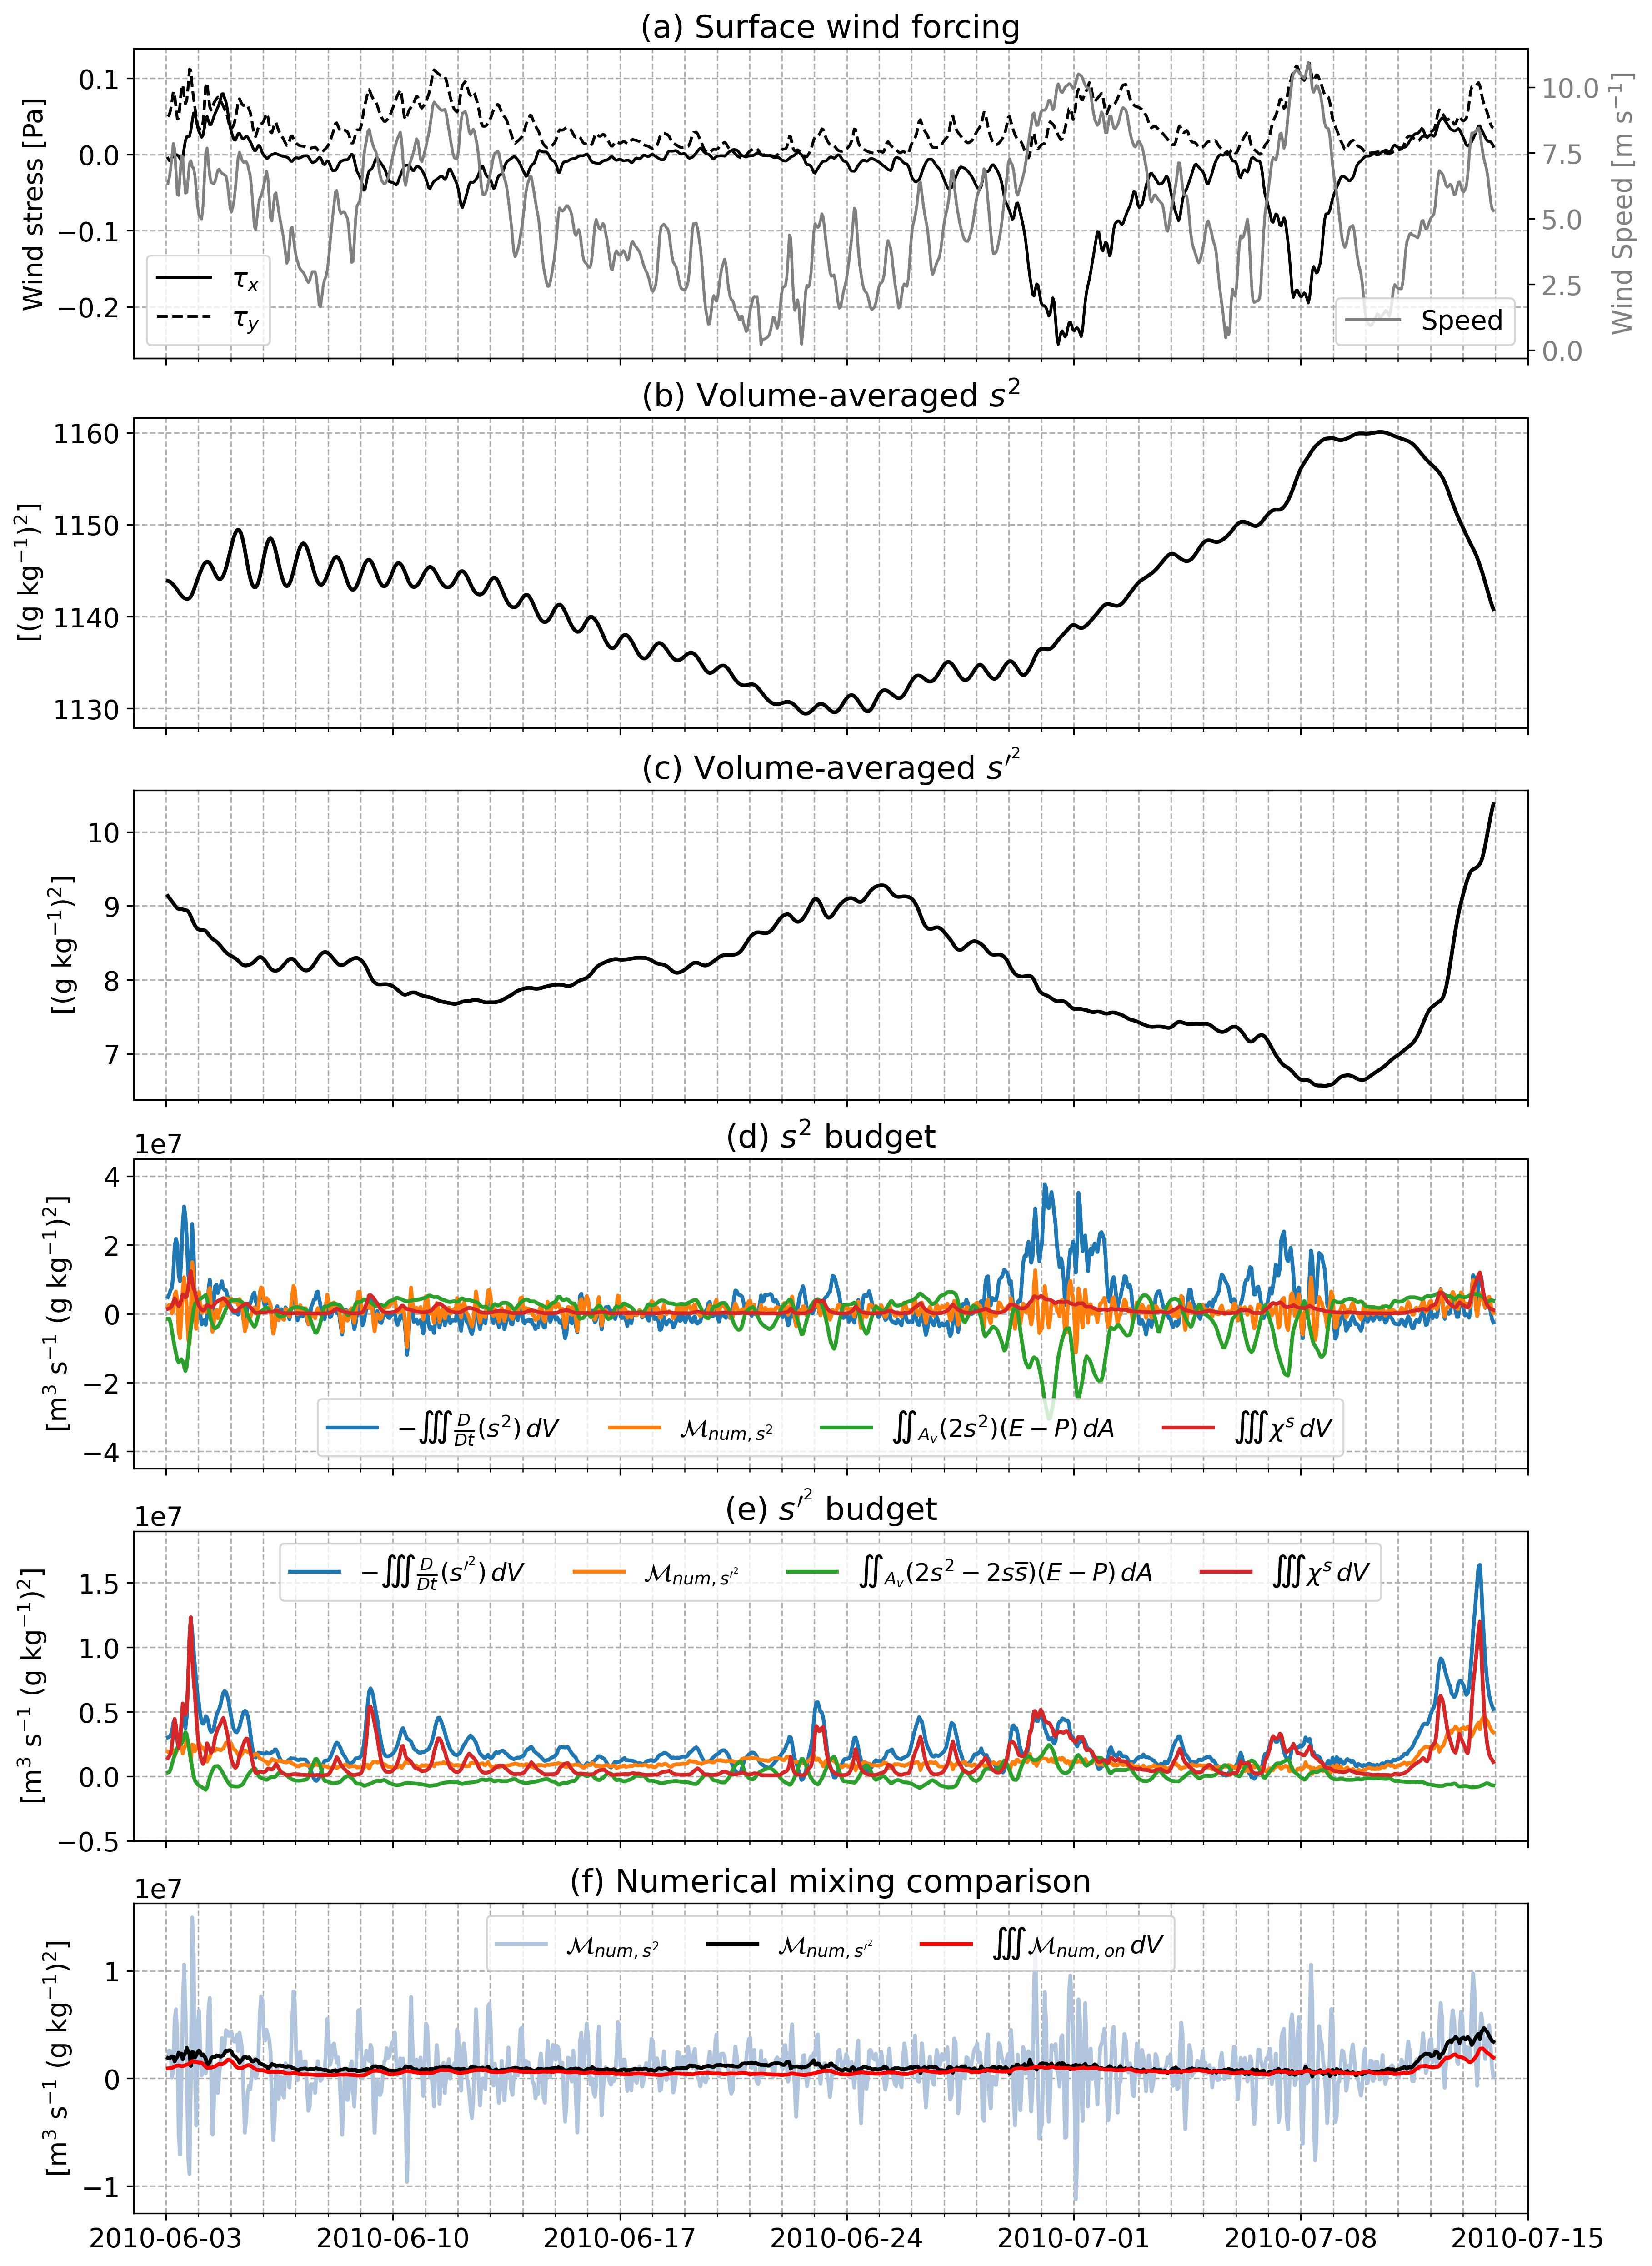
\includegraphics[width = 0.85\linewidth]{figures/james_2023/Figure7_budgets.jpg}}
  \caption{Time series from the coarse simulation averaged over the location of the child grid for east-west wind stress $\tau_x$, north-south wind stress $\tau_y$, and wind speed (a). Volume-averaged $s^2$ (b), volume-averaged $s^{\prime^2}$ (c), volume-integrated $s^2$ budget (d) and $s^{\prime^2}$ budget (e), and comparison between the offline numerical mixing and the online numerical mixing (f). The tendency and advection terms of Eqs. \ref{eq:salt2_vint} and \ref{eq:svar_int} have been combined using the material derivative $\iiint_V \frac{Dc}{Dt} \, dV$, where $c$ denotes the tracer. The horizontal $s^2$ and s$^{\prime^2}$ diffusion terms were omitted from (d) and (e) because they are more than an order of magnitude smaller than the other terms, but are included in their respective numerical mixing calculations.}
  \label{fig:budget_comparison}
\end{figure}

Time series of volume-averaged $s^2$ and $s^{\prime^2}$ (Fig. \ref{fig:budget_comparison} a-b) demonstrate that $s^2\gg s^{\prime^2}$ and that the budgets exhibit a different time dependency. The volume-averaged $s^{\prime^2}$ rarely exceeds $10$ (g kg$^{-1}$)$^2$ and exhibits reduced inertial variability throughout the simulation. The oscillations displayed in the $s^2$ and $s^{\prime^2}$ budgets correspond strongly to the local inertial period ($\sim$ 24 hours) because they are modulated by other variables prone to inertial variability such as the horizontal velocities. Higher frequency oscillations are generated by competition between transient changes in the surface wind field and freshwater input from the M/A rivers. 

For $s^2$ and $s^{\prime^2}$, the advection and tendency terms are highly correlated and have been combined to reduce clutter. Mathematically, this is expressed using the volume integral of their material derivatives and is written as 
\begin{equation}
    \iiint_V \frac{Dc}{Dt} \, dV = \iiint_V \frac{\partial c}{\partial t} \, dV + \iint_{A_l} \mathbf{u}c \cdot \hat{\mathbf{n}} \, dA \quad ,
\end{equation}
 where $c$ is the tracer. Stronger winds are generally associated with larger tendency and advection terms for $s^2$ and $s^{\prime^2}$, which is reflected in their respective material derivatives. The difference between the material derivatives and surface fluxes for $s^2$ and $s^{\prime^2}$ elucidates the influence that removing the volume average salinity has on the dynamics of $s^{\prime^2}$ (Fig. \ref{fig:budget_comparison} c-d). $\iiint \frac{D}{Dt}(s^2) \, dV$ is significantly noisier than $\iiint \frac{D}{Dt}(s^{\prime^2}) \, dV$, which we hypothesize is due the larger numerical error associated with the tendency term, and to a lesser extent, the advection term. The tendency term in the $s^2$ budget is nearly an order of magnitude larger than the $s^{\prime^2}$ budget and will experience larger error because both tendency terms are calculated using the same numerical scheme (i.e., centered finite differences). This error should be reduced by increasing the model output frequency, which we investigate in Section \ref{sec:discussion}. Surface $s^2$ fluxes exert a much larger influence on the $s^2$ budget for much of the simulation, with the physical mixing term often remaining the smallest. The opposite is true for the $s^{\prime^2}$ budget, where the term balance often experiences competition between the physical mixing and the material derivative.  

Estimates of numerical mixing depend strongly on whether $s^2$ or $s^{\prime^2}$ is used, with both offline methods demonstrating significant error with respect to time. $\mathcal{M}_{num, s^2}$ is significantly noisier than $\mathcal{M}_{num, s^{\prime^2}}$ and may exceed the other methods by over an order of magnitude despite the online method being derived in terms of $s$ and $s^2$. Consequently, the $s^2$ budget should not be used for offline quantification of numerical mixing because $\mathcal{M}_{num, s^2}$ does not converge to $\mathcal{M}_{num, s^{\prime^2}}$ for hourly output. $\mathcal{M}_{num, on}$ and $\mathcal{M}_{num, s^{\prime^2}}$ are positive definite, with $\mathcal{M}_{num, s^{\prime^2}}$ almost always overestimating $\mathcal{M}_{num, on}$. The accuracy of $\mathcal{M}_{num, s^{\prime^2}}$ relative to $\mathcal{M}_{num, on}$ is strongly time dependent and the time-averaged $\mathcal{M}_{num, s^{\prime^2}}$ is 60\% larger than the time-averaged $\mathcal{M}_{num, on}$. From June 17-24, the time-averaged $\mathcal{M}_{num, on}$ is 141\% larger than the time-averaged $\mathcal{M}_{num, s^{\prime^2}}$. From July 1-8, however, it is only 12\% larger. These results suggest the offline method is not suitable for accurate quantification of numerical mixing in our model. However, it is unclear whether convergence between $\mathcal{M}_{num, s^2}$, $\mathcal{M}_{num, s^{\prime^2}}$, and $\mathcal{M}_{num,on}$ can be achieved by increasing the output frequency. We discuss possible causes for this, including potential impacts of model output frequency, discretization errors, and other sources of spurious mixing that may contaminate the on- and offline methods in Section \ref{sec:discussion}.  

The effects of the extra terms on the behaviour of the $s^2$ budget are further explored in Fig. \ref{fig:s2_extra_terms}. The volume-averaged salinity changes by less than 1 g kg$^{-1}$ over the simulation and experiences a strong inertial signal until the end of June, after which the inertial signal weakens or vanishes for several days at a time. The differences between the $s^2$ and $s^{\prime^2}$ budgets are generally dominated by competition between $(\partial_t \overline{s}^2)V$ and cross-advective flux $2 \overline{s} \iint (\mathbf{u}s^\prime) \cdot \, dA$ ($r = 0.95$, $p \ll 0.05$). Physically, this relationship shows that in the presence of stratification, the differences between the volume-integrated $s^2$ and $s^{\prime^2}$ budgets is partially modulated by the size of the control volume $V$ ($\partial_t \overline{s}^2$ is small relative to $V$) and the advection of the salinity perturbations through the lateral boundaries. The residual of $(\partial_t \overline{s}^2)V+2 \overline{s} \iint (\mathbf{u}s^\prime) \cdot \hat{\mathbf{n}} \, dA$ is balanced out by the differences in surface fluxes $\iint (2 \overline{s}^2 + 2 \overline{s} s^\prime)(E-P) \, dA$ and the volume-averaged salinity squared times the advection of the flow through the lateral boundaries $\overline{s}^2 \iint \mathbf{u} \cdot \hat{\mathbf{n}} \, dA$. The horizontal cross diffusion term $2 \overline{s} \iiint \nabla_H \cdot (\kappa_H \nabla_H s^{\prime}) \, dV$ remains on average several orders of magnitude smaller than the other terms in the $s^2$ and $s^{\prime^2}$ budgets. This is because the horizontal diffusion terms are small for our model due to prescribed value of $\kappa_H$. Ultimately, all of the extra terms in the $s^2$ budget are linked to $\overline{s}$, with $(\partial_t \overline{s}^2)V$ decreasing in magnitude when amplitude of the inertial variability of $\overline{s}$ decreases. The $\overline{s}^2$ advection term is not as sensitive to the changes in the inertial variability of $\overline{s}$ and oscillates between first and second order, becoming more important at the end of June as $\overline{s}$ begins to increase.

\begin{figure}
 \centerline{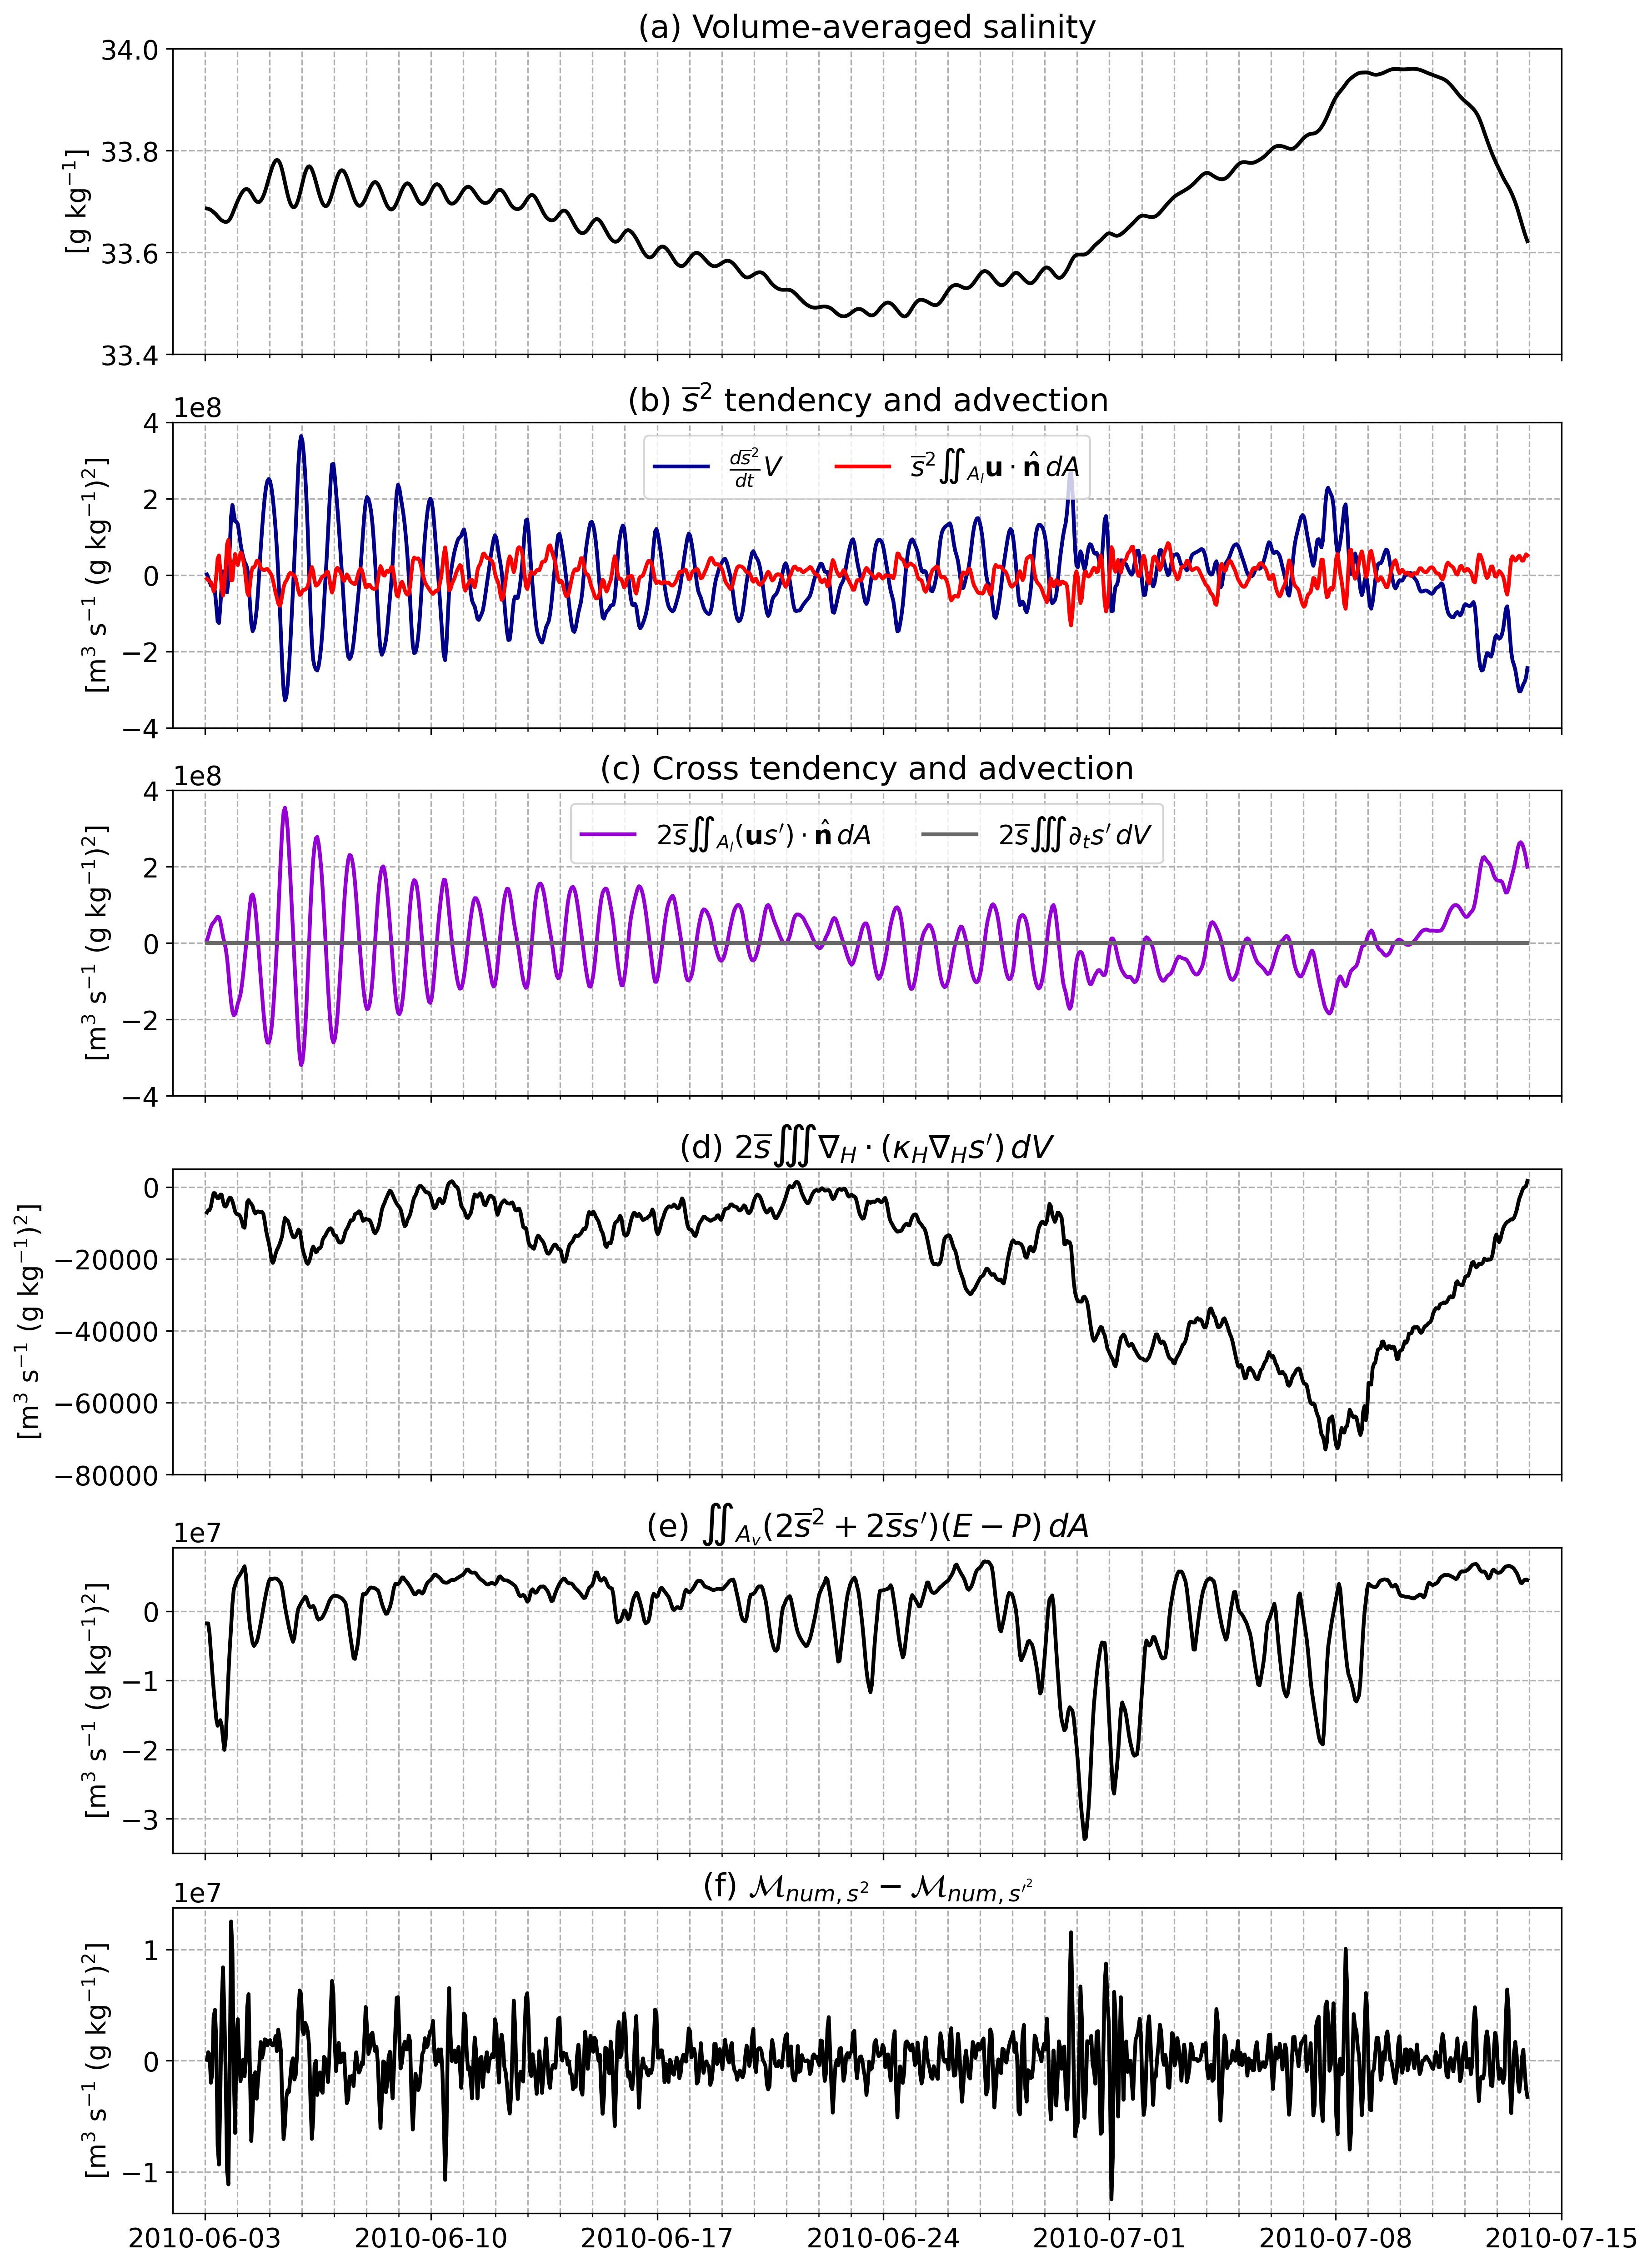
\includegraphics[width = 0.85\linewidth]{figures/james_2023/Figure8_extra_terms.jpg}}
  \caption{Time series from the coarse simulation of the volume-averaged salinity (a) and the balance of the volume-integrated extra terms in the $s^2$ equation given by Eq. \ref{eq:differences}. $\overline{s}^2$ tendency and advection (b), $2 \overline{s} s^\prime$ tendency and advection (c), turbulent horizontal cross diffusion (d), extra $s^2$ surface fluxes (e), and differences between the $s^2$ and $s^{\prime^2}$ numerical mixing $\mathcal{M}_{num, s^2}-\mathcal{M}_{num, s^{\prime^2}}$ (f). $\mathcal{M}_{num, s^2}-\mathcal{M}_{num, s^{\prime^2}}$ yields a large residual that should decrease as model output frequency increases.}
  \label{fig:s2_extra_terms}
\end{figure}

To investigate the bulk impacts of nesting on mixing, Fig. \ref{fig:volume-integrated} displays time series volume-integrated $\chi^s$, $\chi_H^s$, and ratios of fine to coarse $\chi^s$, $\mathcal{M}_{num, on}$, total mixing, and the ratio of $\chi^s$ and $\mathcal{M}_{num, on}$ for both simulations. For the coarse simulation, $\chi_H^s$ comprises 2.3$\%$ of the total physical mixing in the coarse simulation and 5.8$\%$ in the fine simulation. In the coarse simulation, the volume-integrated and time-averaged ratio of numerical to total mixing is 50$\%$. For the fine simulation, this ratio decreases to 32$\%$ because the physical mixing increases and the numerical mixing decreases. The time-averaged physical mixing in the fine simulation is 42$\%$ larger than the coarse simulation and is almost always larger instantaneously, with the greatest disparity occurring during the wind-driven mixing event near July 6 where the fine simulation physical mixing is a factor of four larger than the coarse simulation.  The time-averaged numerical mixing in the fine simulation is 35$\%$ smaller on average relative to the coarse simulation and only grows larger than the coarse numerical mixing at several times. The total mixing in the fine simulation is 14$\%$ larger on average than the coarse simulation, but exhibits large temporal variability and may be twice as large or reduced by a third compared to the coarse simulation. During the first three weeks of June, the total mixing in the fine simulation may be more of less than the coarse simulation due to reduced numerical mixing, but for the remainder of the simulation the relative increase in physical mixing generally exceeds the decrease in numerical mixing. A striking comparison is the ratio of numerical to physical mixing. The numerical mixing is larger than the physical mixing in the coarse simulation for a significant portion of the simulation due to the strong inertial variability in the physical mixing, at several times over half an order of magnitude larger. However, this ratio is significantly reduced in the fine simulation. 

\begin{figure}
 \centerline{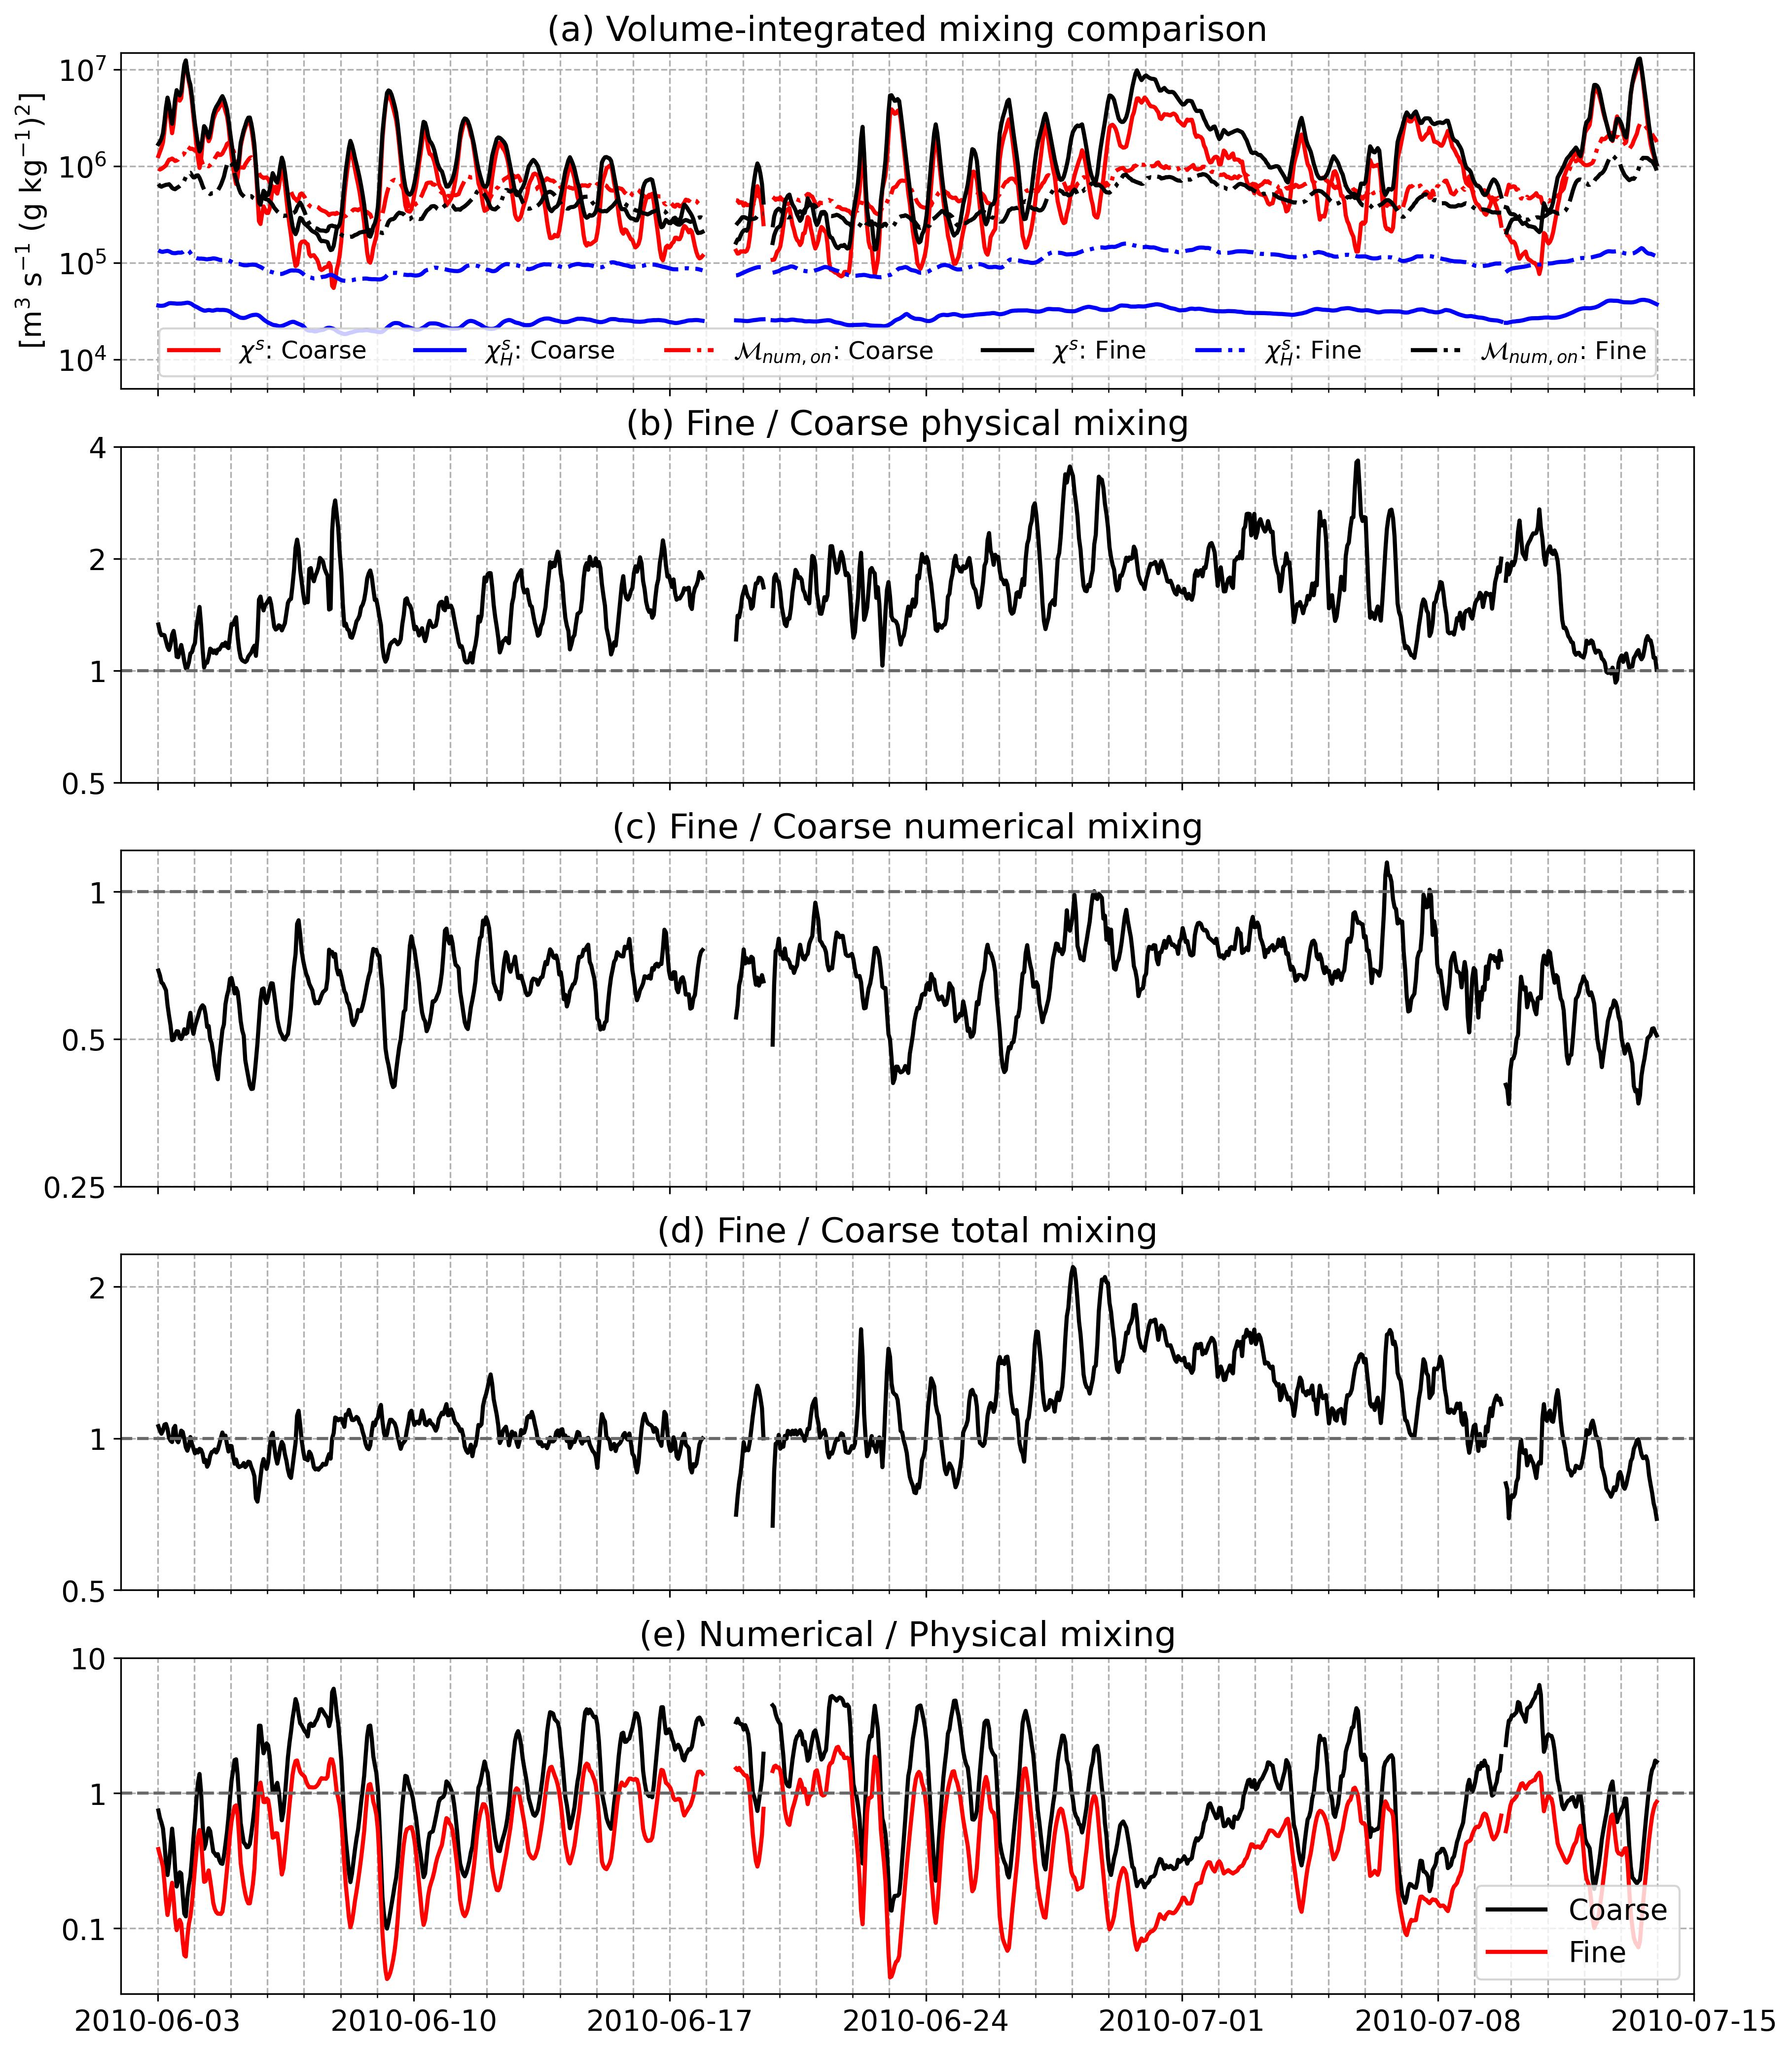
\includegraphics[width = 0.9\linewidth]{figures/james_2023/Figure9_vintegrated.jpg}}
  \caption{Time series of volume-integrated $\chi^s$, $\chi_H^s$,  and $\mathcal{M}_{num, on}$ for the coarse and fine simulations (a). All plots below are derived from these values, displaying fine/coarse physical mixing (b), fine/coarse numerical mixing (c), fine/coarse total mixing (d), and numerical/physical mixing for both models (e). Missing values seen in the time series correspond to output lost during the restart process of the fine simulation and were removed from the parent simulation offline for direct comparison. Note each plot is on a log scale of base 10 or base 2.}
  \label{fig:volume-integrated}
\end{figure}

\section{Discussion} \label{sec:discussion}

We find that numerical mixing constitutes a significant fraction of the total mixing -- the sum of physical and numerical mixing -- and exceeds the physical mixing for much of the simulation due to strong lateral salinity gradients generated by freshwater input from the Mississippi and Atchafalaya rivers.

Our analysis of the offline tracer budgets suggests the $s^2$ budget may overestimate the online numerical mixing by over an order of magnitude (Fig. \ref{fig:budget_comparison}). Building on the work of \citet{Wang_2021}, we hypothesized that the differences are primarily due to errors associated with the tendency term of each tracer and can be reduced by increasing the model output frequency. To test our hypothesis and examine whether $\mathcal{M}_{num, s^2}$ will converge to $\mathcal{M}_{num, s^{\prime^2}}$, we performed two additional numerical simulations of the coarse model with output frequencies of 30- and 10 minutes (twice and six times finer than the native resolution, respectively). The results of the simulations are summarized in Fig. \ref{fig:mixing_time_series} and discussed in Sections \ref{sec:s2_online_conv}-\ref{sec:sprime2_online_conv}.

\begin{figure}[h]
 \centerline{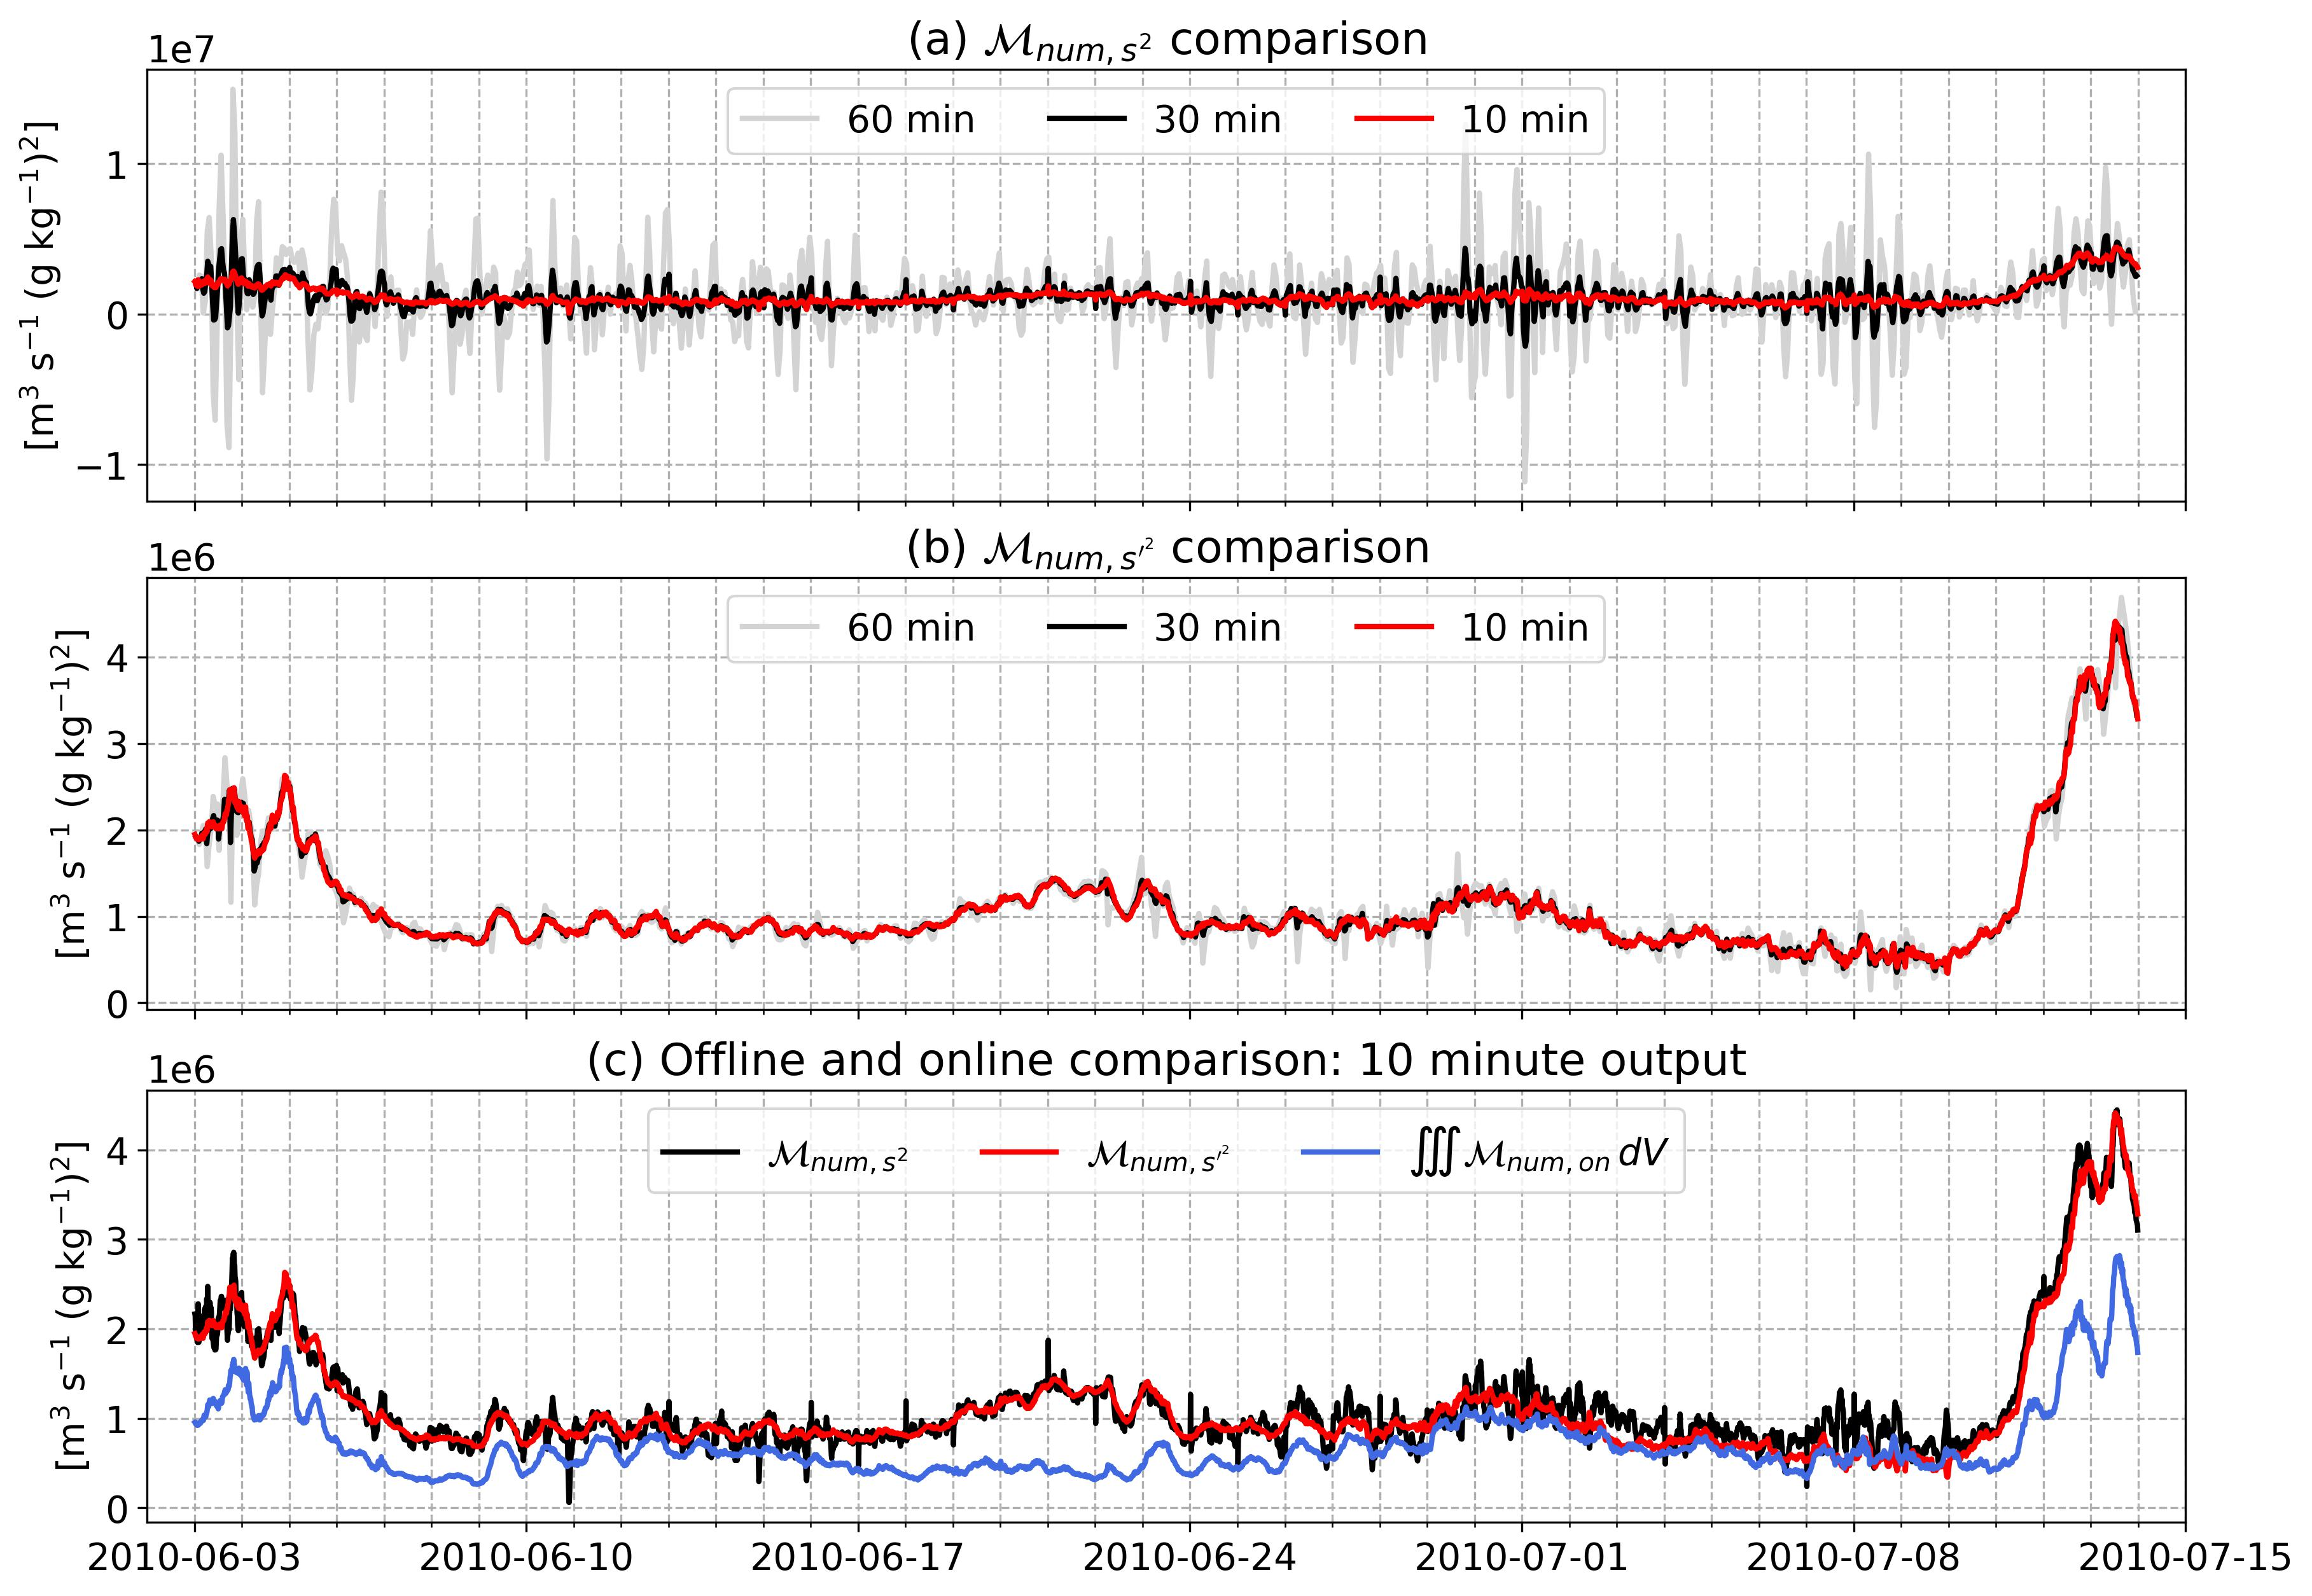
\includegraphics[width = \linewidth]{figures/james_2023/Figure10_output_freq.jpg}}
  \caption{Time series for the coarse simulation for model output frequencies of 60 minutes, 30 minutes, and 10 minutes of $\mathcal{M}_{num, s^2}$ (a) and $\mathcal{M}_{num, s^{\prime^2}}$ (b). Comparison of 10 minute output $\mathcal{M}_{num, s^2}$, $\mathcal{M}_{num, s^{\prime^2}}$, and volume-integrated $\mathcal{M}_{num, on}$  (c).}
  \label{fig:mixing_time_series}
\end{figure}

Additionally, the local and volume-integrated numerical mixing constitute significant fractions of the total mixing, even when the model resolution is increased to $\mathcal{O}(300)$ m in a two-way nested simulation. Despite the time-averaged spatially-integrated numerical mixing decreasing in the fine simulation by 35\%, Fig. \ref{fig:cross_section} suggests that numerical mixing may be occasionally enhanced at the grid-scale. Numerical mixing is dependent on a number of factors, including the magnitude of the horizontal salinity gradients, grid resolution, model timestep, and the representation of dynamical processes. \citet{Wang_2021} suggested that numerical mixing is proportional to the square of the horizontal salinity gradients, however they did not demonstrate that this relationship is robust for higher order and more complex advection schemes. We find, based on Figs.~\ref{fig:surface_pdfs} and~\ref{fig:whole_pdfs} that, on average, the salinity gradients do not increase significantly in the fine simulation, but there are more instances of high values of relative vorticity, divergence, and strain. Even when considering the increased horizontal mixing in the fine simulation, the results suggest that different physical processes have emerged in the fine simulation. We discuss the relationship between horizontal resolution, numerical mixing, and model processes in Section \ref{sec:salinity_gradient_mag}. 

\subsection{Convergence between $\mathcal{M}_{num, s^2}$ and $\mathcal{M}_{num, s^{\prime^2}}$}
\label{sec:s2_online_conv}

As the output frequency increases, $\mathcal{M}_{num,s^2}$ beings to converge towards $\mathcal{M}_{num,s^{\prime^2}}$ but still remains noisy, with the two in much better agreement for the 10 minute output simulation. However, we find this insufficient because 10 minute output is impractical for long-term coastal ocean simulations at this time. To test our hypothesis that the higher inaccuracy associated with $\mathcal{M}_{num, s^2}$ is primarily due to errors associated with the tendency term $\iiint_V \partial_t s^2 \, dV$, we down-sampled the 10 minute output of the $s^2$ budget to match the 30 minute output. After rearranging Eq. \ref{eq:salt2_vint}, the residual term balance can be written as 
\begin{equation} \label{eq:downsampled_termbalance}
    \begin{split}
    \Delta \mathcal{M}_{num, s^2} = -\Delta \textrm{Tendency}-\Delta \textrm{Advection}+\Delta \textrm{Surface $s^2$ flux}-\Delta \textrm{Physical mixing} \\
    + \Delta \textrm{Horz. diff.} \quad ,
    \end{split}
\end{equation}
where $\Delta = \gamma_{30}-\gamma_{10}$, with $\gamma$ denoting the terms in the volume-integrated $s^2$ budget and the subscripts referring to the model output frequency in minutes. The difference in the estimate of numerical mixing due to differences in model output frequency is given by $\Delta \mathcal{M}_{num, s^2}$. 

We computed the covariance between each term in Eq. \ref{eq:downsampled_termbalance} and $\Delta \mathcal{M}_{num, s^2}$ divided by the variance of $\Delta \mathcal{M}_{num, s^2}$ to test the significance of each term, which we denote by the variable $q$. This provides an estimate of the fraction of the variance in $\Delta \mathcal{M}_{num, s^2}$ explained by each term. For $-\Delta$Tendency, $q = 1.271$ and for $-\Delta$Advection, $q = -0.270$, indicating that $\Delta$Tendency will over-predict $\Delta \mathcal{M}_{num, s^2}$, whereas $-\Delta$Advection will compensate for this over-prediction. When combined, $q = 1.001$, indicating that $\Delta$Physical Mixing, $\Delta$Surface flux, and $\Delta$Horz. Diff. do not significantly contribute to $\Delta \mathcal{M}_{num, s^2}$, which is because they are orders of magnitude smaller relative to $\Delta$Tendency and $\Delta$Advection. $\Delta$Advection is also significant, but to a lesser extent than $\Delta$Tendency because the horizontal velocities are highly unsteady and therefore sensitive to model output frequency. The physical mixing is computed online and remains more periodic relative to $\Delta$Tendency and $\Delta$Advection, so it is less sensitive to model output frequency. Likewise, the freshwater flux $(E-P)$ has an temporal resolution of several hours that is linearly interpolated prior to the calculation of $\Delta$Surface flux, so it is unsurprising it remains insignificant. $\Delta$Horz. diff. does not change signficantly because the horizontal $s^2$ diffusion is well under an order of magnitude smaller than the other terms in the volume-integrated $s^2$ budget. These results were consistent with scatter plots of $\Delta \mathcal{M}_{num, s^2}$ and the RHS terms of Eq. \ref{eq:downsampled_termbalance} (not shown). 

\subsection{Convergence between $\mathcal{M}_{num,s^{\prime^2}}$ and $\mathcal{M}_{num,on}$}
\label{sec:sprime2_online_conv}

For 10 minute output, $\mathcal{M}_{num,s^{\prime^2}}$ becomes slightly less noisy but the general structure remains unchanged and unconditional convergence (i.e., for all times) is not achieved. Interestingly, convergence does not substantially improve as output frequency increases, especially during the last week of the simulation when the largest physical and numerical mixing occurs (Fig. \ref{fig:budget_comparison} d). 

There are a number of factors that could cause the difference between on- and offline estimates of numerical mixing, and many of them are difficult to quantify. First, we cannot say with certainty that $\mathcal{M}_{num, on}$ will yield identical results whether $s$ or $s^{\prime}$ is computed locally despite our analysis with a 1D upwind scheme. Another source of error is our use of lower-order accurate discretizations for offline analysis of the tracer variance budgets (see \ref{Appendix:offline_method}). For example, ROMS has implemented several higher order internal time-stepping schemes for tracers since its inception (e.g., third-order Adams-Bashforth), whereas we use a first order centered finite difference for time derivatives in the $s^2$ and $s^{\prime^2}$ budgets. Likewise, we used volume-conserving fluxes in the calculation of the $s^2$ and $s^{\prime^2}$ boundary advection instead of reconstructing the MPDATA scheme offline. These discretization errors may be further compounded by our use of average files compared to snapshots.

The reason for this is the offline method is intended to focus on practicality. Recreating a model's complex numerical schemes offline may be more cumbersome than coding the online method into the source code and rerunning it if computational resources are not a concern. Other sources of error are the numerical diffusion of $s^2$ and $s^{\prime^2}$ through the lateral boundaries of the control volume or the generation of spurious convection. Quantification of numerical diffusion would require estimating a numerical diffusion coefficient and as we have shown, we cannot guarantee an offline calculation will be robust. The situation is similar regarding the quantification of spurious convection. 

The online method should be used as the reference due to the lack of convergence and influence of discretization errors associated with the offline method. We can say that increasing the model output frequency will marginally improve the offline estimates, and that the $s^{\prime^2}$ budget will generally yield more accurate estimates of the numerical mixing than the $s^2$ budget, especially at low output frequency. In our case, $\mathcal{M}_{num, s^{\prime^2}}$ almost always overestimates $\mathcal{M}_{num, on}$ and qualitatively captures the temporal variability well. However, there is no guarantee this will be the case for other ocean models. Therefore, we cannot recommend the offline method for generic analysis of numerical mixing because it does not converge even at impractically-high output frequencies and we are unable to identify the exact reasons for the lack of convergence. These issues may be compounded for larger-scale ocean models. The proper output variables would have to be chosen before running the simulation and the output frequency will be decreased for larger-scale models. Future research could potentially improve the offline method by using more higher-order numerical schemes for the tendency and advection terms, but this would have to be tested on a per-model basis and referenced against an online benchmark for validation.

\subsection{Relating numerical mixing to $|\nabla_H s|$ and other processes} \label{sec:salinity_gradient_mag}

As shown in Fig. \ref{fig:cross_section}, numerical mixing may be over an order of magnitude larger than the physical mixing in regions with strong density gradients, generally corresponding to areas of larger $|\nabla_H s|$. \citet{Smolarkiewicz_1983} showed that after discretizing a one-dimensional advection equation with a first-order upwind scheme, the numerical mixing $\mathcal{M}_{num, up}$ is
\begin{equation} \label{eq:mnum_approx}
    \mathcal{M}_{num, up} = |u|\Delta x (1-C) \bigg(\frac{\partial s}{\partial x} \bigg)^2 \sim |u|\Delta x \bigg(\frac{\partial s}{\partial x} \bigg)^2 \quad ,
\end{equation}
where $|u|$ is the magnitude of the constant horizontal velocity, $\Delta x$ is the horizontal grid resolution, $C=\frac{u \Delta t}{\Delta x}$ is the Courant number with online time step $\Delta t$. After rearranging, it can be shown that the right-hand-side of Eq. \ref{eq:mnum_approx} is formulated such that the numerical mixing is equal to an implicit diffusion coefficient $|u|\Delta x-u^2 \Delta t$ multiplied by the square of the horizontal salinity gradients. As \citet{Wang_2021} notes, when the Courant number is less than one, the numerical mixing is approximately proportional to the square of the horizontal salinity gradients. \citet{Wang_2021} applied this equation to a realistic simulation of the Changjiang River plume using two tracer advection schemes (MPDATA and Third-order Upstream-biased Horizontal Scheme) and suggested that this relationship holds true qualitatively (their Figs. 8-9). 

We further investigate the relationship between $\mathcal{M}_{num, on}$ and $(\nabla_H s)^2 = (\partial_x s)^2+(\partial_y s)^2$ in Fig. \ref{fig:mnum_sgrad}, which shows weighted histograms of the absolute value of $\mathcal{M}_{num, on}$ and $(\nabla_H s)^2$ in log$_{10}$ space, weighted by grid cell volume $dV$, for the coarse and fine simulations. We performed a weighted linear regression analysis to test the robustness of the two-dimensional form of Eq. \ref{eq:mnum_approx}. There is a clear log-log relationship between $\mathcal{M}_{num, on}$ and $(\nabla_H s)^2$ ($r^2=0.55$ for coarse simulation, $r^2=0.39$ for the fine simulation). To test for a power law dependence, we conducted an empirical linear fit of $\mathcal{M}_{num, on}$ and $(\nabla_H s)^2$ in log$_{10}$ space, which slightly improved the fit ($r^2=0.60$ for coarse simulation, $r^2=0.46$ for the fine simulation). The relatively high $r^2$ suggest that the horizontal salinity gradients could be used to roughly approximate the numerical mixing, even for higher order and more complex advection schemes.

\begin{figure}
 \centerline{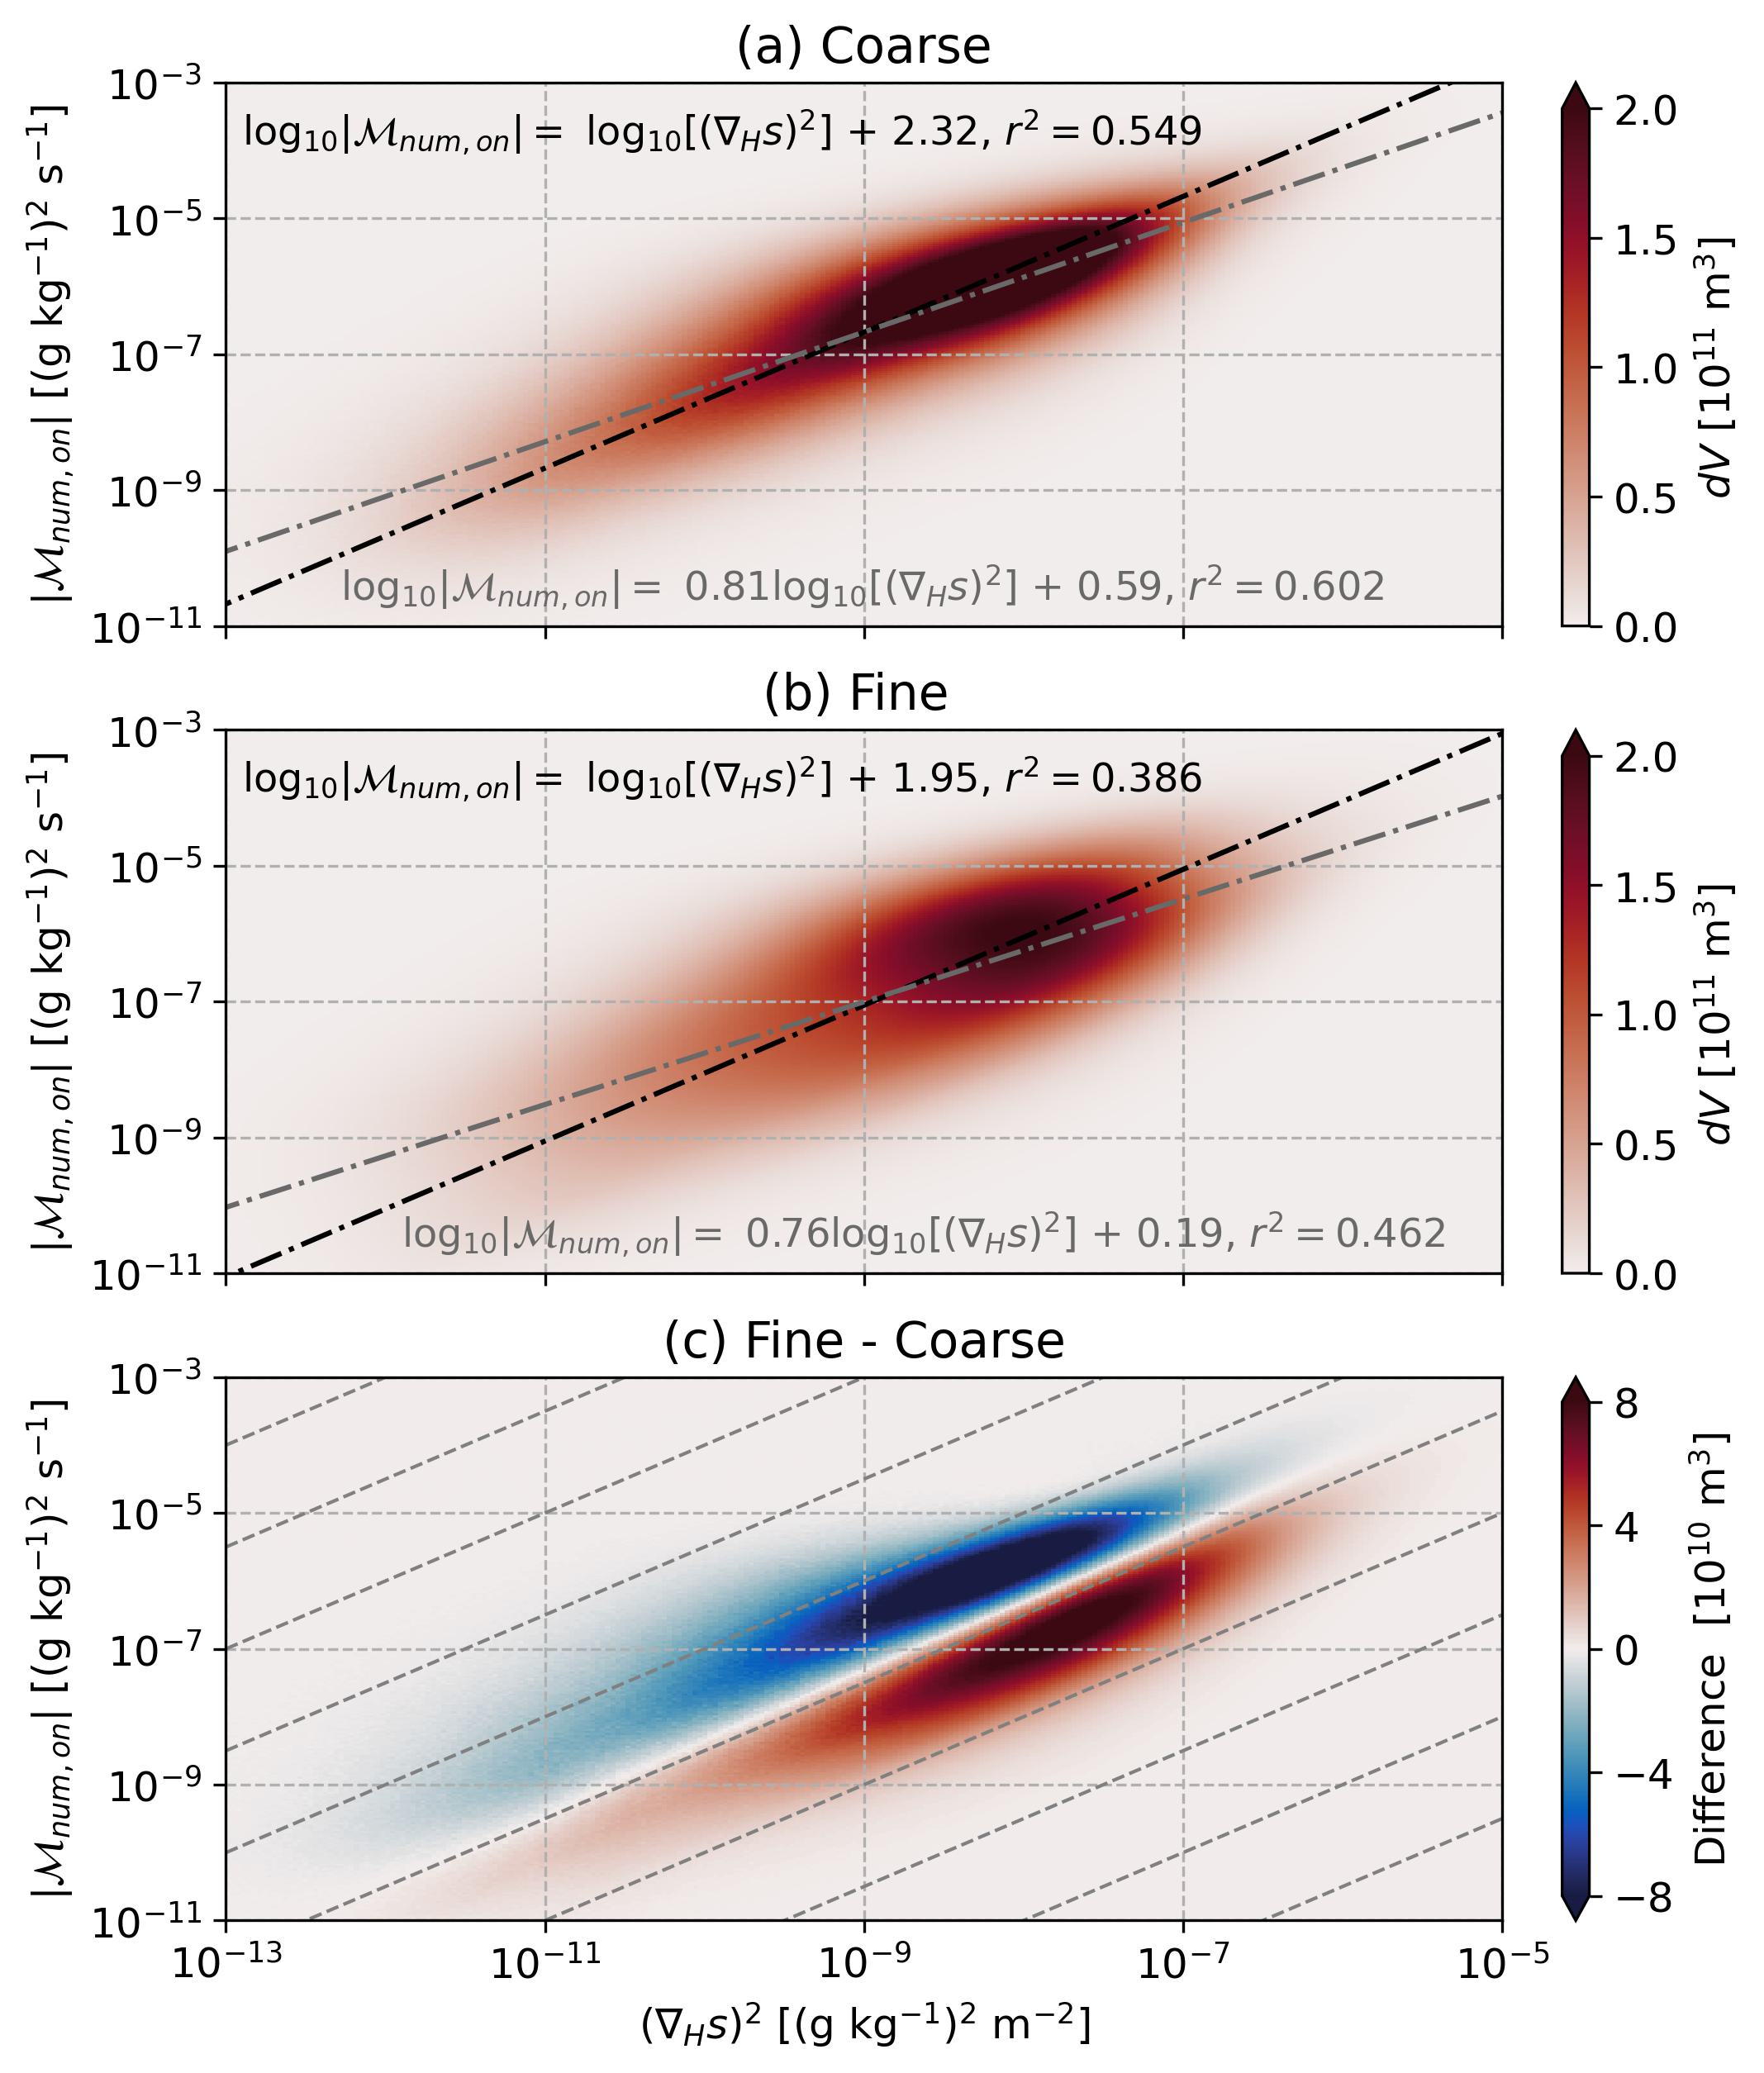
\includegraphics[width =0.9\linewidth]{figures/james_2023/Figure11_sgradmag_histogram.jpg}}
  \caption{Histograms of the horizontal salinity gradient squared $(\nabla_H s)^2$ and absolute value of online numerical mixing $|\mathcal{M}_{num, on}|$ weighted by grid cell volume $dV$ for the coarse (a) and fine (b) simulations, and their differences (c). The thick dashed lines in (a)-(b) display weighted linear regression results for the approximate two-dimensional form of Eq. \ref{eq:mnum_approx} (black) and an empirical fit in log-log space (gray). The regressions and weighted coefficients of determination were obtained by subsampling the coarse grid model every three $\xi,\eta$ points and the fine simulation every 15 points for the entire simulation period. The thick dashed gray lines in (c) indicate a slope of 1.}
  \label{fig:mnum_sgrad}
\end{figure}

As $(\nabla_H s)^2$ increases, more of the domain volume is concentrated at larger values of $\mathcal{M}_{num, on}$. The relationship begins to taper off at $(\nabla_H s)^2 \sim \mathcal{O}(10^{-6})$ g$^2$ kg$^{-2}$ m$^{-2}$, corresponding to salinity gradients associated with surface fronts and the pycnocline in the M/A river plume. These fronts have strong salinity gradients and numerical mixing, but they occupy a small portion of the water column, hence the decrease in grid cell volume. Weaker salinity gradients are associated with longer length and time scales and are correlated with weaker numerical mixing. 

The differences between the coarse and fine simulations demonstrate that the fine simulation has weaker numerical mixing distributed at stronger salinity gradients than the coarse simulation. In other words, for a given salinity gradient, the fine simulation will experience less numerical mixing on average compared to the coarse simulation. The dividing line separating the positive and negative changes to $dV$ between the simulations has a slope of nearly one, suggesting that the change in numerical mixing is proportional to $(\nabla_H s)^2$. The coefficient of determination is lower in the fine simulation because the numerical mixing depends not only on $|\nabla_H s|$, but the components of grid resolution $dV$, water velocities, and the model timestep. In the fine simulation, $\Delta x$ and $\Delta y$ decreased by a factor of five, but the time-averaged volume-integrated numerical mixing decreases by only 35$\%$, suggesting a nonlinear relationship between numerical mixing, the square of the horizontal salinity gradients, and horizontal grid resolution. Although identifying the exact dynamical feedbacks that cause this non-linearity to arise is beyond the scope of this paper, an analysis (not shown) of the instability angle $\phi_{{Ri}_b}$ derived in \citet{Thomas_2013} (their Eq. 8) suggests that the fine simulation is more susceptible to symmetric and inertial instabilities than the coarse simulation. Coupled with the sharp changes of the velocity gradient tensor but insignificant changes to $|\nabla_H s|$ in Figs. \ref{fig:surface_pdfs}-\ref{fig:whole_pdfs}, this is consistent with the idea that different dynamical processes emerge as the resolution is increased, which complicates the relationship between horizontal resolution and numerical mixing. However, had $|\nabla_H s|$ increased significantly, this would have increased the numerical mixing in the fine simulation.

\section{Summary and conclusions} \label{sec:conclusions}

We have studied physical and numerical mixing in a numerical model of the Texas-Louisiana (TXLA) continental shelf using a combination of on- and offline methods based on salinity variance. Physical mixing is defined as the dissipation of salinity variance associated with numerical closure schemes and numerical mixing is defined as the mixing generated by the discretization of salinity advection. Salinity variance can be defined in terms of salinity squared $s^2$ and volume-mean salinity variance $s^{\prime^2}$. Previous research \citep{Burchard_2019, MacCready_2018, Qu_2022_box} has shown the residuals of the $s^2$ and $s^{\prime^2}$ budgets can be used to estimate numerical mixing. However, the robustness of the offline method in realistic simulations has only been assessed qualitatively by \citet{Wang_2021}. The online method, which locally calculates numerical mixing $\mathcal{M}_{num, on}$ as the difference between the advected salinity squared and the square of the advected salinity divided by the model timestep \citep{Burchard_2008}. $\mathcal{M}_{num, on}$ is used to evaluate the accuracy of the offline method. 

We find the residuals of the $s^2$ and $s^{\prime^2}$ budgets, $\mathcal{M}_{num, s^2}$ and $\mathcal{M}_{num, s^{\prime^2}}$, do not converge to the online method. This is true even as the model output frequency is increased to 10 minutes, an impractical output frequency for long-term realistic coastal models at this time. The $s^2$ budget at hourly output may miscalculate numerical mixing by over an order of magnitude. During the study period, $s^2\gg s^{\prime^2}$, which causes the resulting tendency and advection terms in the $s^2$ budget to be over an order of magnitude larger than the $s^{\prime^2}$ budget. We derive the $s^2$ budget in terms of volume-averaged salinity $\overline{s}$ and salinity perturbation $s^\prime$ to relate $\mathcal{M}_{num, s^2}$ and $\mathcal{M}_{num, s^{\prime^2}}$ and investigate the consequences of this scaling. We find the $s^2$ budget experiences larger truncation error compared to the $s^{\prime^2}$ budget when using identical numerical schemes. $\mathcal{M}_{num, s^2}$ begins to converge to $\mathcal{M}_{num, s^{\prime^2}}$ as output frequency increases but is still noisy at 10 minute output. The scaling of $s^2$ and $s^{\prime^2}$ over the shelf is quite different than previous estuarine models \citep{Li_2018, Li_2021, Warner_2020}, where $s^{\prime^2}$ may be similar in scale to $s^2$ since estuary domains include a transition from fresh river water to background coastal salinities. 

The time-averaged $\mathcal{M}_{num, s^{\prime^2}}$ is 60\% larger than the time-averaged $\mathcal{M}_{num, on}$. Although $\mathcal{M}_{num, s^{\prime^2}}$ is much less sensitive to model output frequency, it does not converge to $\mathcal{M}_{num, on}$ for all times and cannot be considered robust. There are many sources of uncertainty that could contaminate the on- and offline methods. For example, a mismatch between our model's in- and external schemes for calculating time derivatives or additional sources of spurious mixing such as grid-scale noise in velocity. 

Consequently, we cannot recommend the offline method for generic quantification of numerical mixing. Although \citet{Wang_2021} qualitatively showed success in estimating numerical mixing offline, we find offline mixing estimates to be inaccurate, and only useful in providing a rough sense and scale of the numerical mixing. Despite this, the offline method qualitatively captures the larger signals in the temporal variability well and might be informative to researchers who are unable to use an online method. We also feel the approach might be useful in comparing different scenarios where the primary questions are about the relative magnitude of numerical mixing. This is particularly relevant for estuarine and coastal models already using a high model output frequency and spatial resolution, but less so for larger-scale models that employ a lower output frequency. 

It is also clear that sources of uncertainty need to be evaluated on a per-model basis, so offline calculation cannot be generally recommended as a primary approach. Given the strong advection and weak physical mixing during summer in the nGoM, we think that our domain is particularly challenging for accurate offline calculation of numerical mixing, and is a good demonstration of the weaknesses of the offline approach. Other regions with relatively stronger physical mixing, e.g., partially mixed estuaries, may be more suitable to the offline approach. However,  a comprehensive understanding of when an offline approach may be feasible is outside the scope of the present study, and so for now we feel the offline approach must be treated as suspect for a particular region until demonstrated otherwise.

Regarding the online analysis, the numerical mixing remains significant relative to the physical mixing even for a submesoscale-resolving coastal ocean model. We find the volume-integrated numerical mixing comprises 57$\%$ of the bulk physical mixing. Instantaneously, the volume-integrated numerical mixing may exceed the physical mixing by almost half an order of magnitude, motivating us to use a two-way nested model with five times the native horizontal grid resolution to examine the sensitivity of numerical mixing to horizontal resolution. We find that the time-averaged volume-integrated numerical mixing decreases by approximately 35$\%$ in the fine simulation, suggesting a nonlinear relationship between horizontal resolution and numerical mixing. Building on the work of \citet{Wang_2021}, we use weighted property histograms to show that numerical mixing is approximately proportional to the square of the horizontal salinity gradients $(\nabla_H s)^2$. As horizontal resolution increases, this relationship weakens because newly resolved dynamical processes emerge, which are evident in histograms of the velocity gradient tensor and $|\nabla_H s|$.  
The salinity field and flow structure for the control volume examined here are dominated by interactions between a rich field of submesoscale eddies, sharp fronts, and strong near-inertial currents. It is encouraging that increasing the horizontal grid resolution decreases the numerical mixing and increases the physical mixing, but at significant computational expense. Another key question resulting from this work is how do changes in numerical and physical mixing at the grid-scale affect the evolution of the mean flow and tracer fields for estuarine and coastal models? We expect numerical mixing to be significant in other realistic simulations of coastal flows, which is particularly relevant for researchers focusing on submesoscale processes, where the impacts of grid-scale numerical mixing are more likely to be pronounced.

\section{Data availability statement} 
All TXLA model output used in this study is publicly available at \url{https://hafen.geos.tamu.edu/thredds/catalog/catalog.html} under the ``TXLA ROMS nested model for SUNRISE/2010" subdirectory. The corresponding analysis code is available at \url{https://doi.org/10.5281/zenodo.7566722}. The calculations were performed in Python ver. 3.9 using the xarray \citep{hoyer_stephan_2021_5771208}, xgcm \citep{abernathey_ryan_p_2022_6643579}, and xroms \citep{xroms} packages. More information about specific packages used for analysis can be found in the code repository. 

% \newpage
% \section{References}
% % % %%% Manually add references after each section
% \bibliographystyle{apalike}
% \begingroup
% \renewcommand{\section}[2]{}%
% \bibliography{references.bib}
% \endgroup